\section{Architettura}

In questa sezione descriviamo brevemente l'architettura del sistema \progetto.

L'architettura adottata è \gloss{event-driven}: ogni componente è isolato e asincrono,
e comunica interfacciandosi e scambiandosi messaggi tramite il broker Apache Kafka.

Il sistema si divide principalmente in tre insiemi di componenti:

\begin{itemize}
    \item Producers
    \item Gestore Personale
    \item Consumers
\end{itemize}

\subsection{Producers}
Il Producer è il componente che resta in ascolto degli webhook provenienti dal suo applicativo specifico (e.g. Redmine, GitLab).
Ha lo scopo di immettere i messaggi su Kafka in formato JSON, conservando solo i campi di interesse e aggiungendone eventualmente di propri.

Al momento della stesura di questo manuale, i Producer implementati sono due:
\begin{itemize}
    \item RedmineProducer
    \item GitlabProducer
\end{itemize}

L'algoritmo di invio dei messaggi differirà solamente nella modalità in cui verrà formato il messaggio finale: per questo motivo abbiamo deciso di utilizzare
il design pattern \gloss{Template Method} per l'implementazione dell'algoritmo. Le classi concrete avranno esclusivamente il compito di implementare
il parser degli Webhook e il metodo del Producer \texttt{webhook\_kind()}.


% \begin{figure}[H]
%     \centering
%     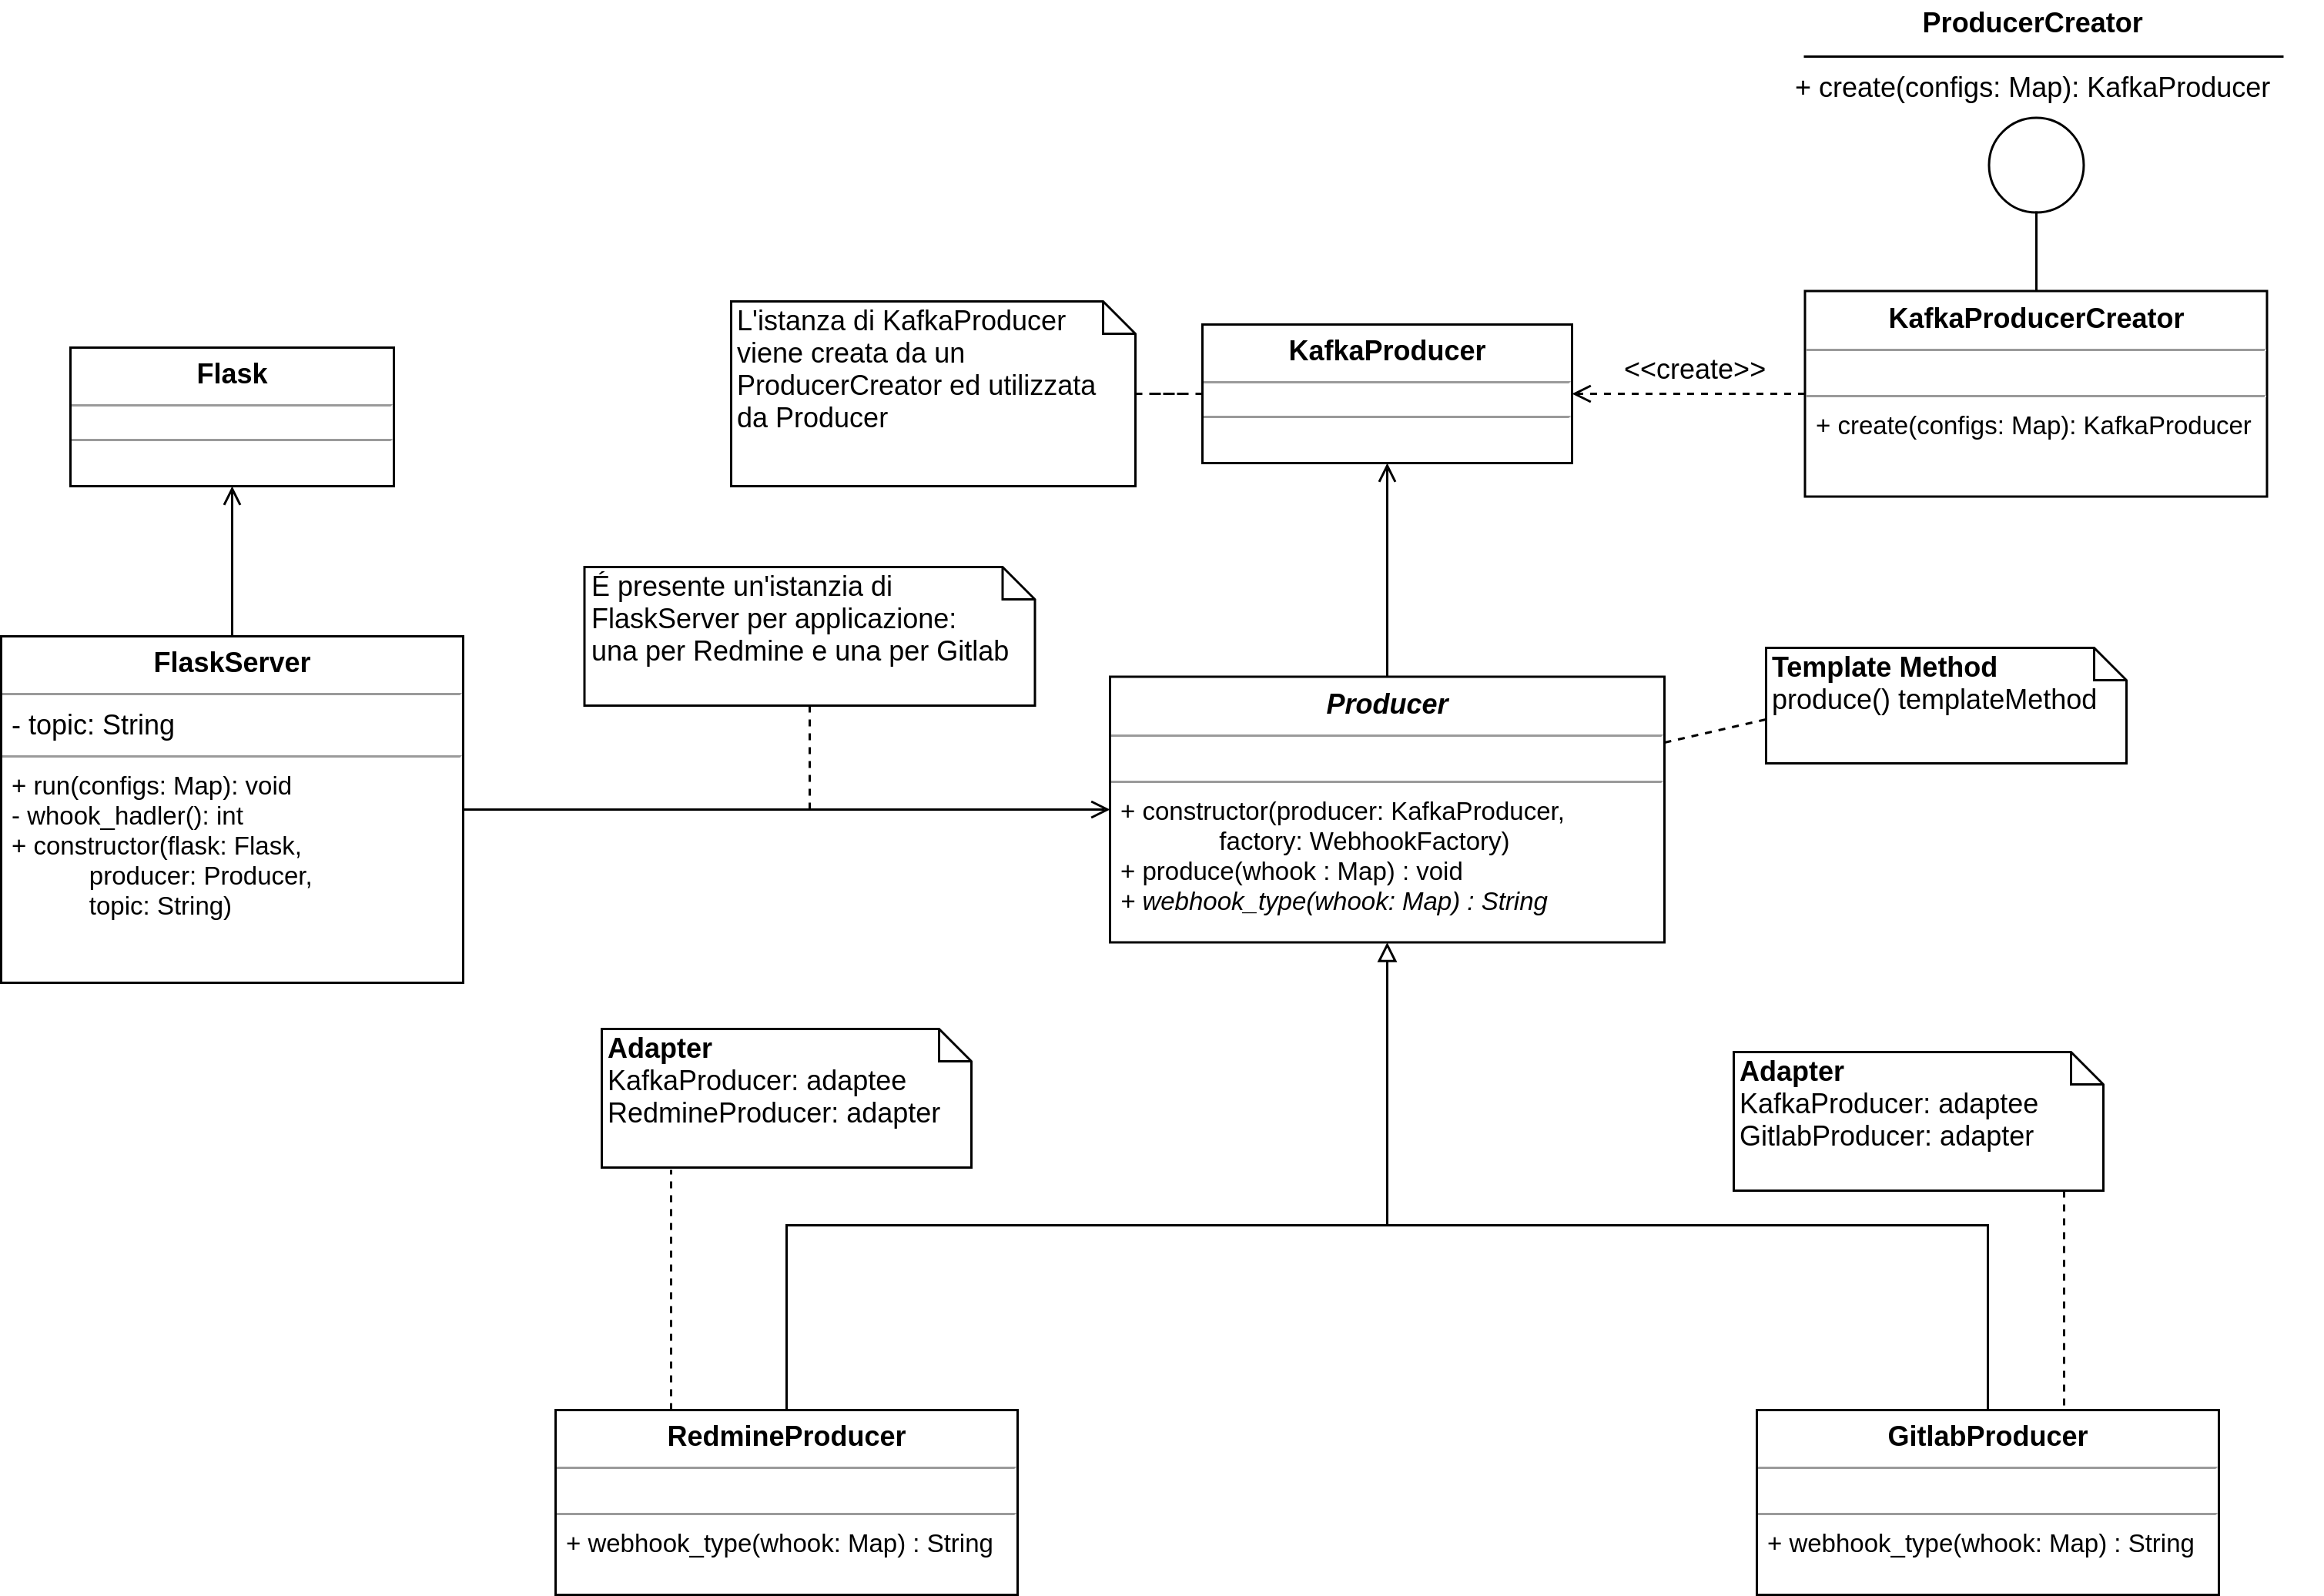
\includegraphics[width=\textwidth]{img/Producers.png}\\
%     \caption{Visione generale dei Producers}
%     \label{fig:producers}
% \end{figure}


\subsubsection{RedmineProducer}

Il Producer di Redmine si occupa di ascoltare gli webhook provenienti dai progetti di Redmine che hanno configurato la porta relativa al componente,
e di immettere nella coda \textit{redmine} di Kafka i messaggi.

Nel seguente diagramma di sequenza è possibile vedere il flusso di esecuzione, che parte dall'arrivo di un webhook da Redmine e si conclude con
l'inoltro del messaggio sulla coda \textit{redmine} di Kafka.

\begin{figure}[H]
    \centering
    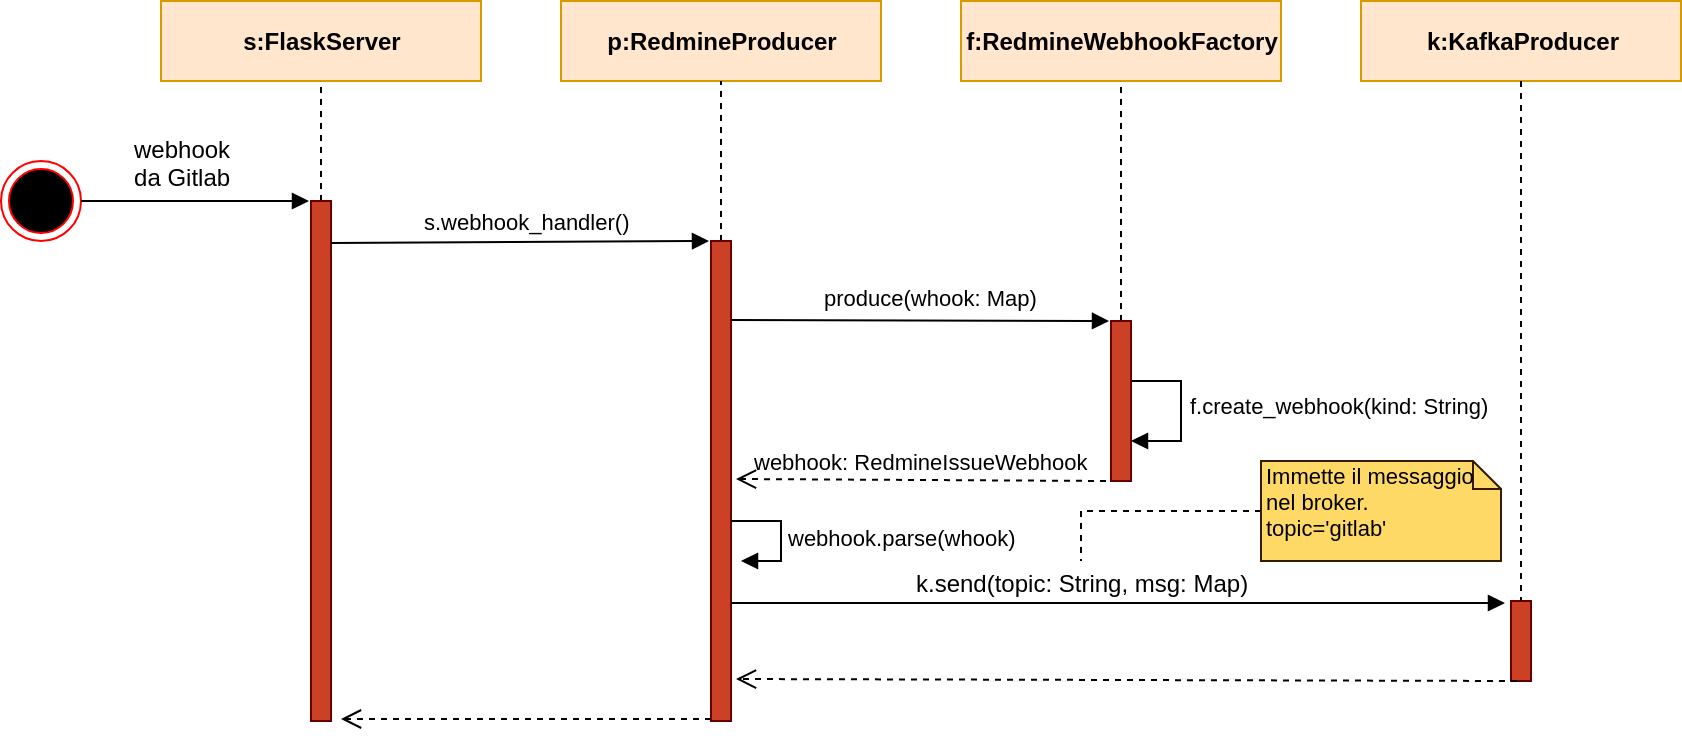
\includegraphics[width=\textwidth]{img/Producer-MsgRedmine.png}\\
    \caption[Diagramma di sequenza di RedmineProducer]{Diagramma di sequenza per la ricezione di un messaggio su RedmineProducer e invio del messaggio su Kafka}
    % \label{fig:producers}
\end{figure}

\paragraph{Diagramma dei package}

Il package \texttt{producer} ha tre dipendenze esterne:
\begin{itemize}
    \item \texttt{Flask}, classe concreta del package di libreria \texttt{flask}: è il server che si mette in ascolto degli webhook provenienti da Redmine.
    \item \texttt{KafkaProducer}, classe concreta del package di libreria \texttt{kafka}: ha il compito di interfacciarsi con il broker Kafka e di immettere
        in esso i messaggi. È costruito su di esso un \gloss{Adapter}, in cui KafkaProducer viene adattato all'astrazione \texttt{Producer}.
    \item Package \texttt{webhook}: ha il compito di effettuare il parsing dei messaggi in entrata.
\end{itemize}

\begin{figure}[H]
    \centering
    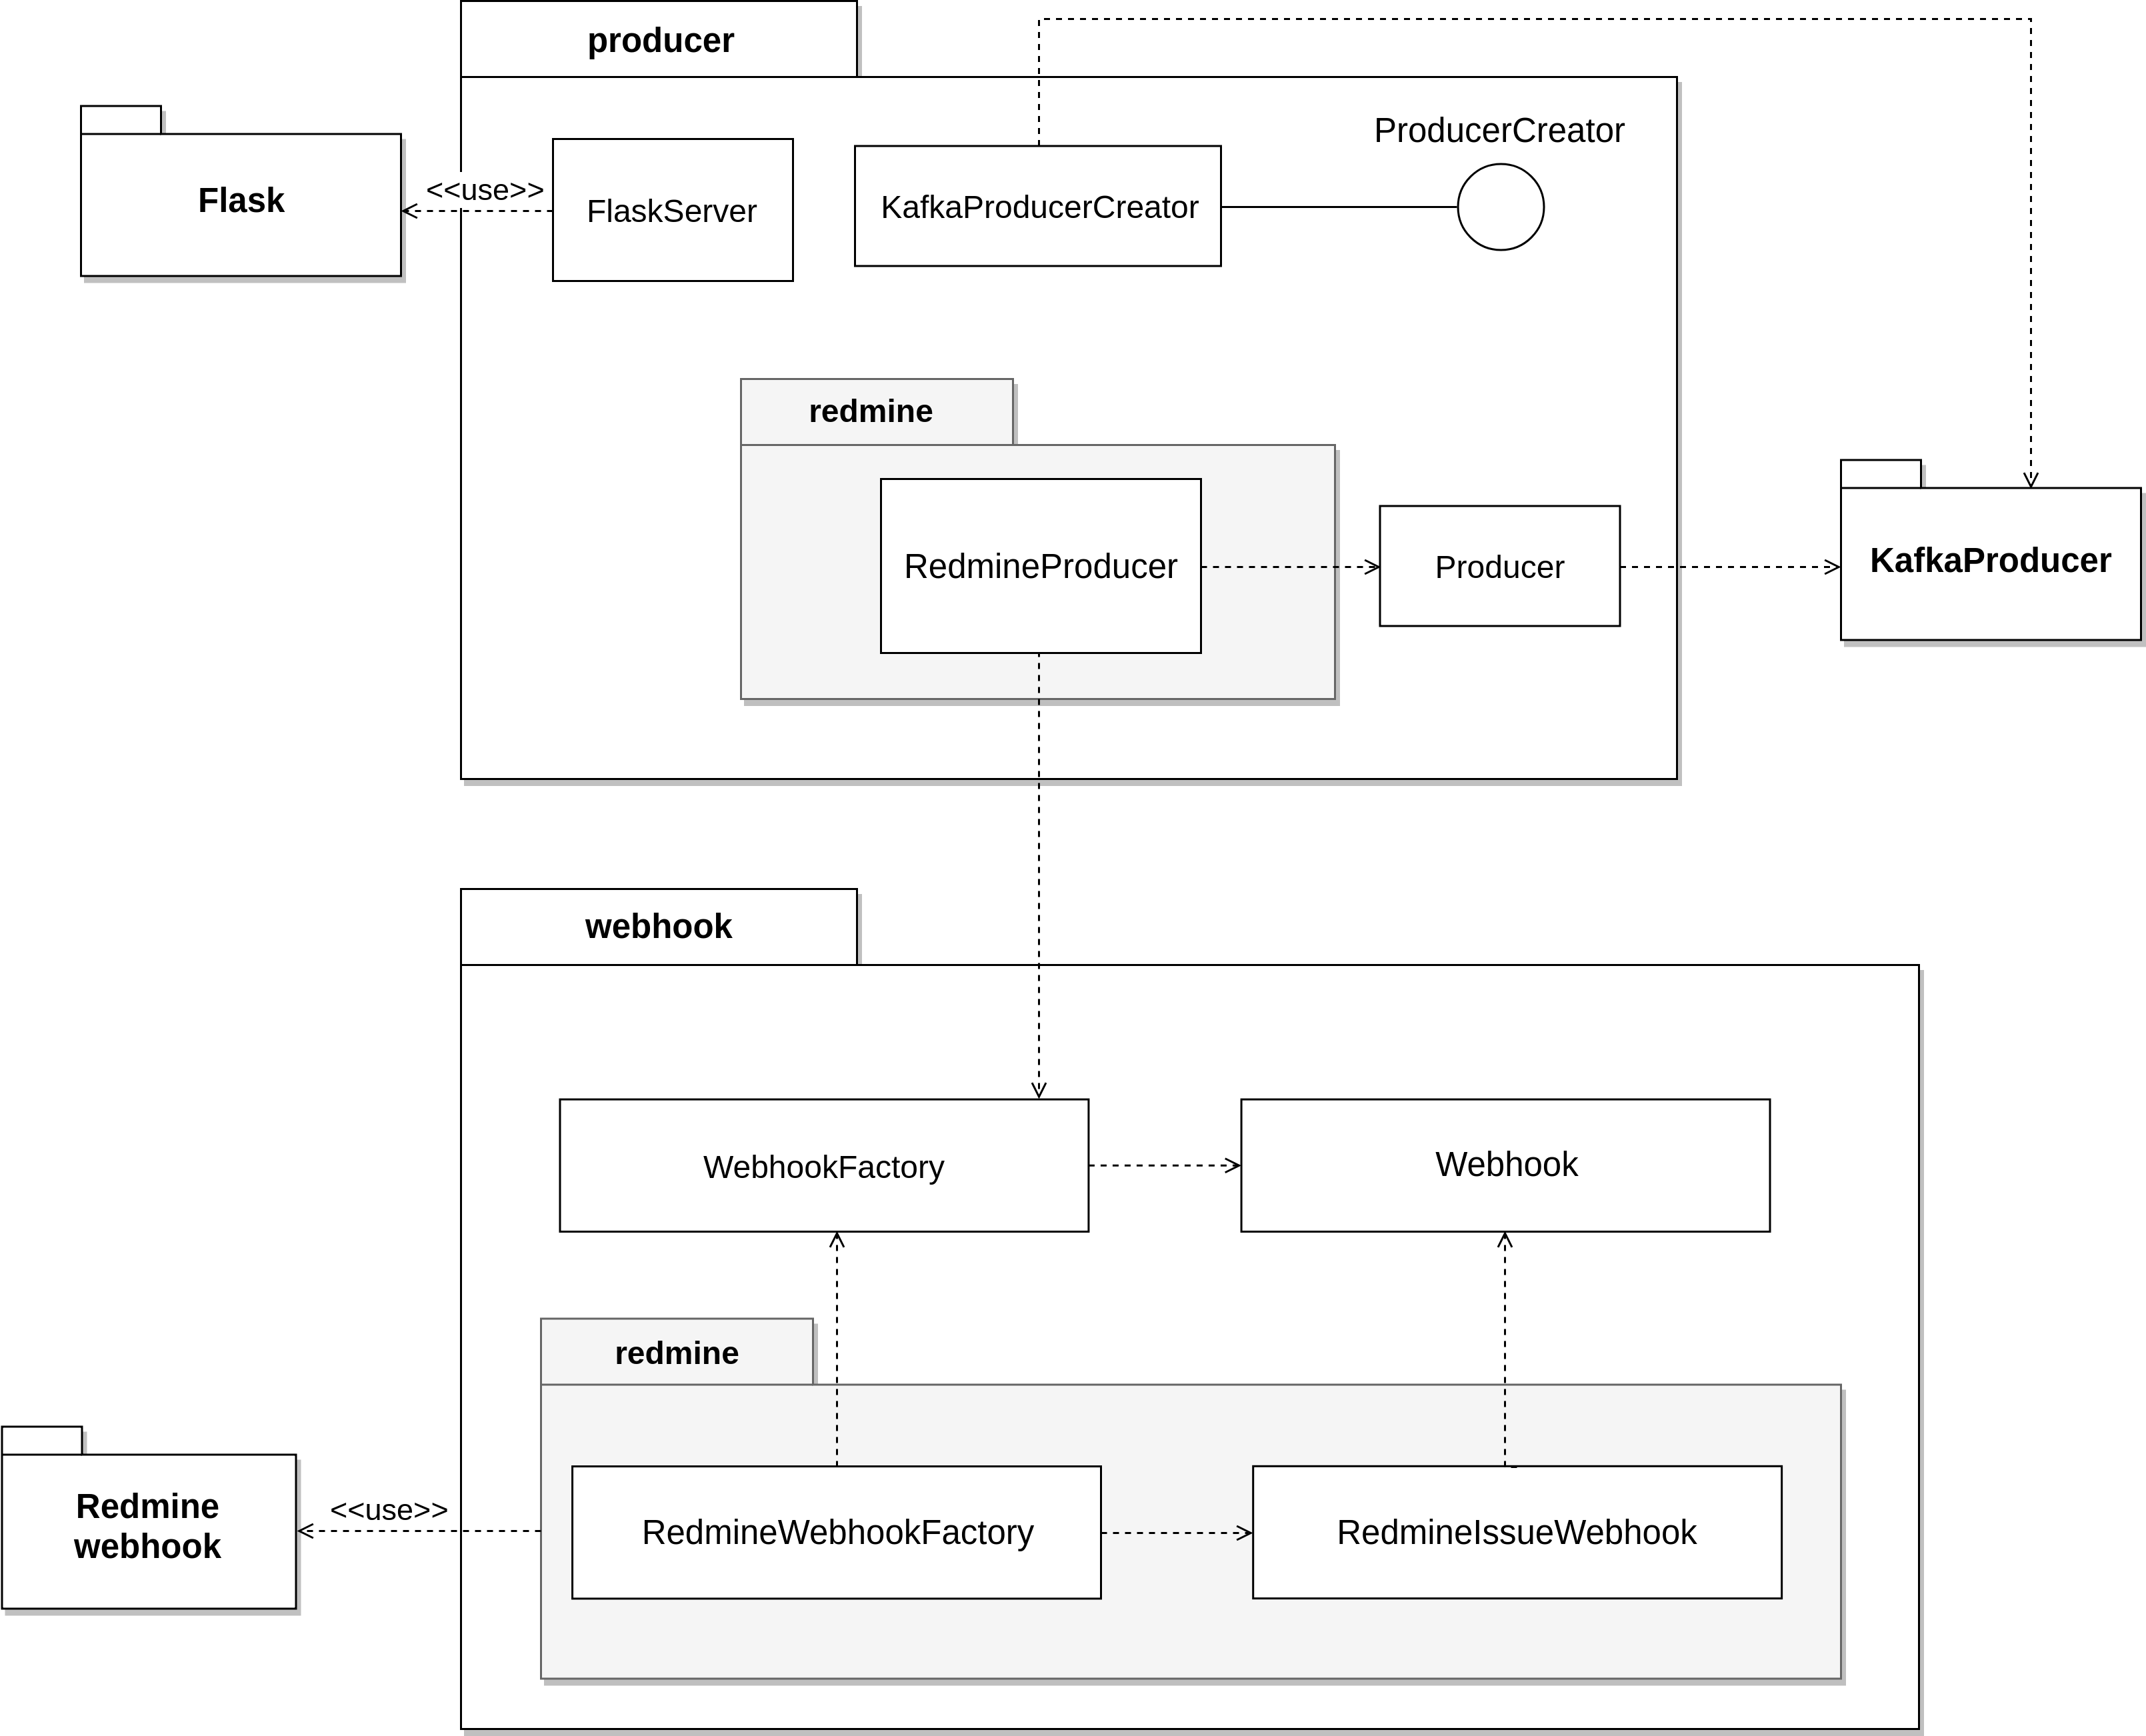
\includegraphics[width=\textwidth]{img/Package-RedmineProducer.png}\\
    \caption{Diagramma dei package di RedmineProducer}
    % \label{fig:producers}
\end{figure}

\paragraph{Diagramma delle classi}

\begin{figure}[H]
    \centering
    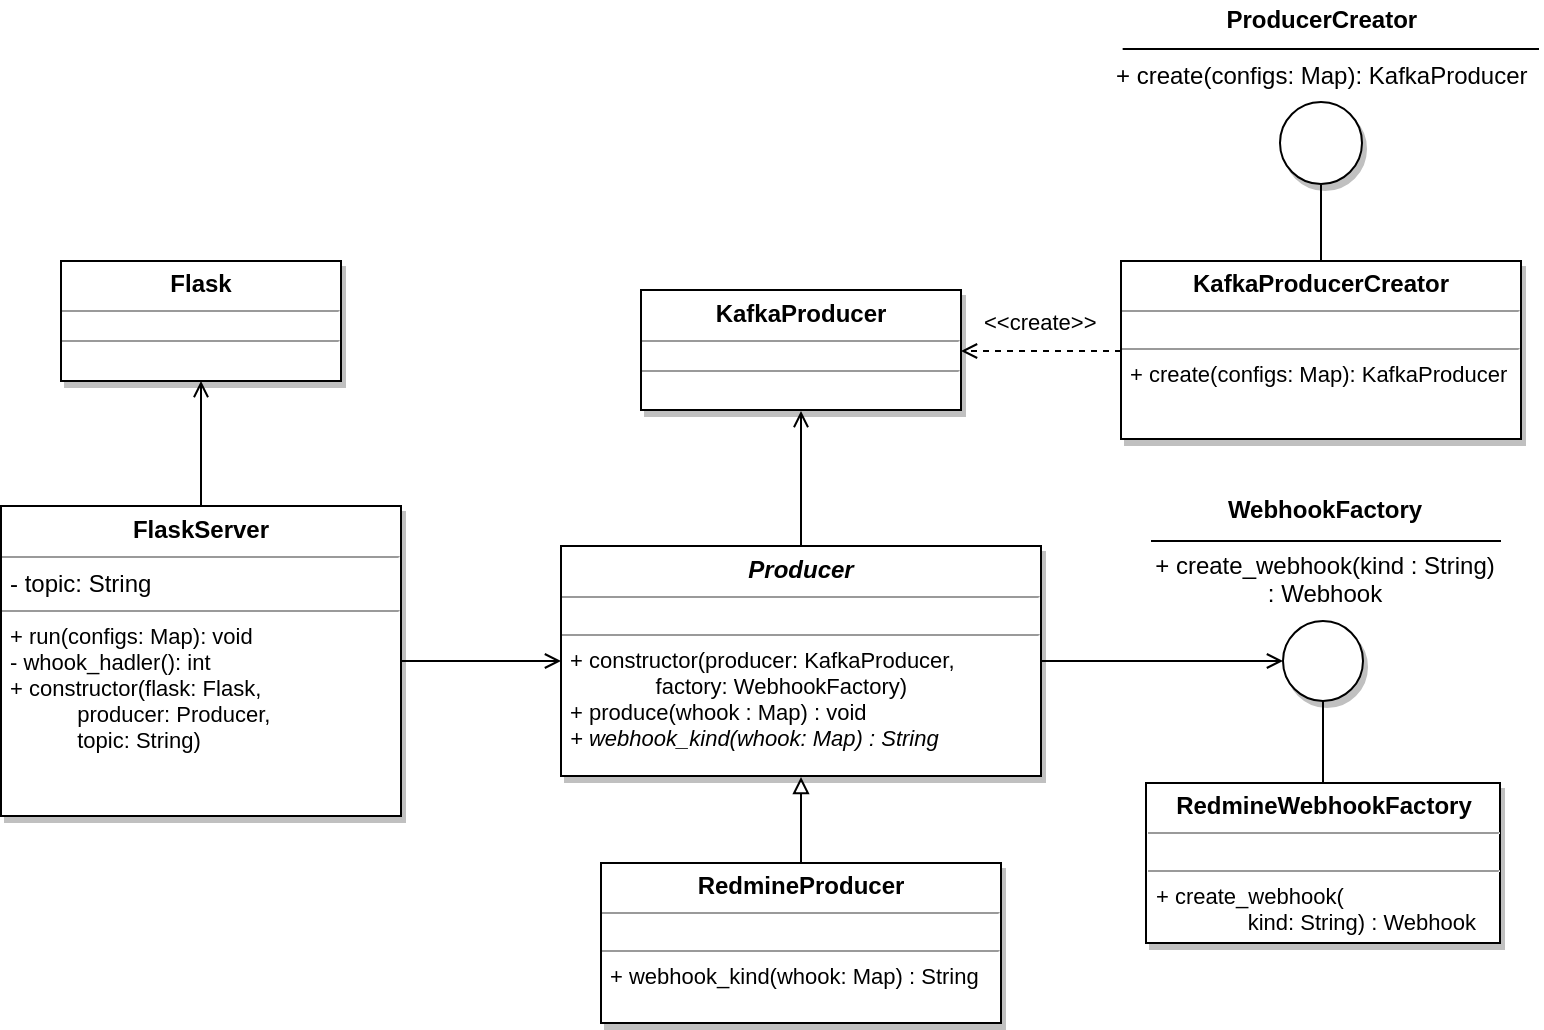
\includegraphics[width=\textwidth]{img/Producers-RedmineProducer.png}\\
    \caption{Diagramma delle classi di RedmineProducer}
    % \label{fig:producers}
\end{figure}

Per fare il parsing dei webhook, \texttt{RedmineProducer} si appoggia alla gerarchia \texttt{Webhook}.
Ogni istanza di \texttt{RedmineProducer} ha un riferimento a una \texttt{WebhookFactory}: quando viene
catturato un webhook da Redmine, chiama il metodo \texttt{create\_webhook(kind)} della
factory associata, passandogli come parametro la tipologia di webhook, in formato stringa.

Essa si occuperà di creare il parser di webhook adeguato al messaggio in entrata.
La classe concreta derivata da Webhook costruisce il messaggio con i campi di interesse da
immettere nella coda di Kafka, e lo restituisce al Produer.

Per Redmine, è presente una sola tipologia di webhook. Tenendo a mente la \gloss{open world assumption},
è stata implementata la gerarchia relativa ai Webhook per permettere agli sviluppatori di poter facilmente
aggiungerne di nuovi.

\begin{figure}[H]
    \centering
    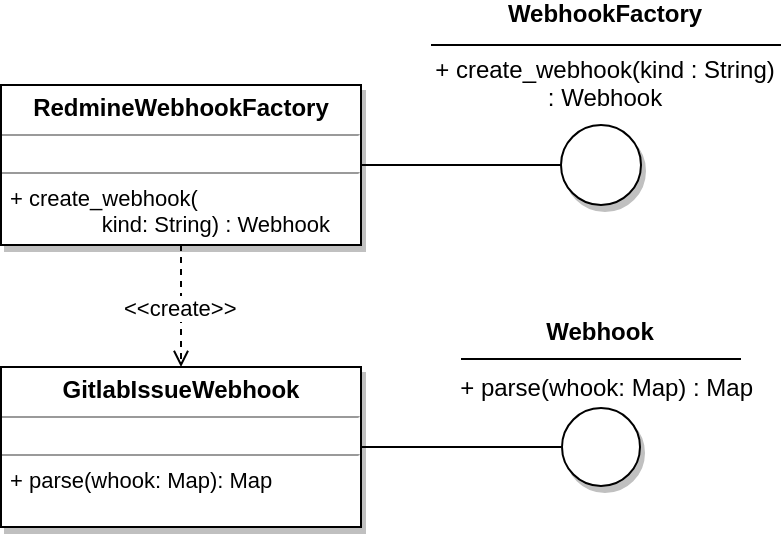
\includegraphics[width=0.6\textwidth]{img/Producers-RedmineWebhook.png}\\
    \caption{Diagramma delle classi di RedmineWebhookFactory}
    % \label{fig:producers}
\end{figure}



\subsubsection{GitlabProducer}
Il Producer di GitLab si occupa di ascoltare gli webhook provenienti dai progetti di GitLab
che hanno configurato la porta relativa al componente, e di immettere nella coda gitlab di
Kafka i messaggi.

Esso è implementato allo stesso modo di quello di Redmine, per cui non verrà ripetuta l'analisi delle
funzionalità che sono identiche al Producer di Redmine. Per tenere totalmente separate e isolate
le componenti, i diagrammi sono stati totalmente separati, anche se le classi risiedono nello stesso package.
Sarà compito dei \gloss{Dockerfile} copiare solamente i file necessari al componente specifico per poter mantenere
isolato il container.


\paragraph{Diagramma dei package}

\begin{figure}[H]
    \centering
    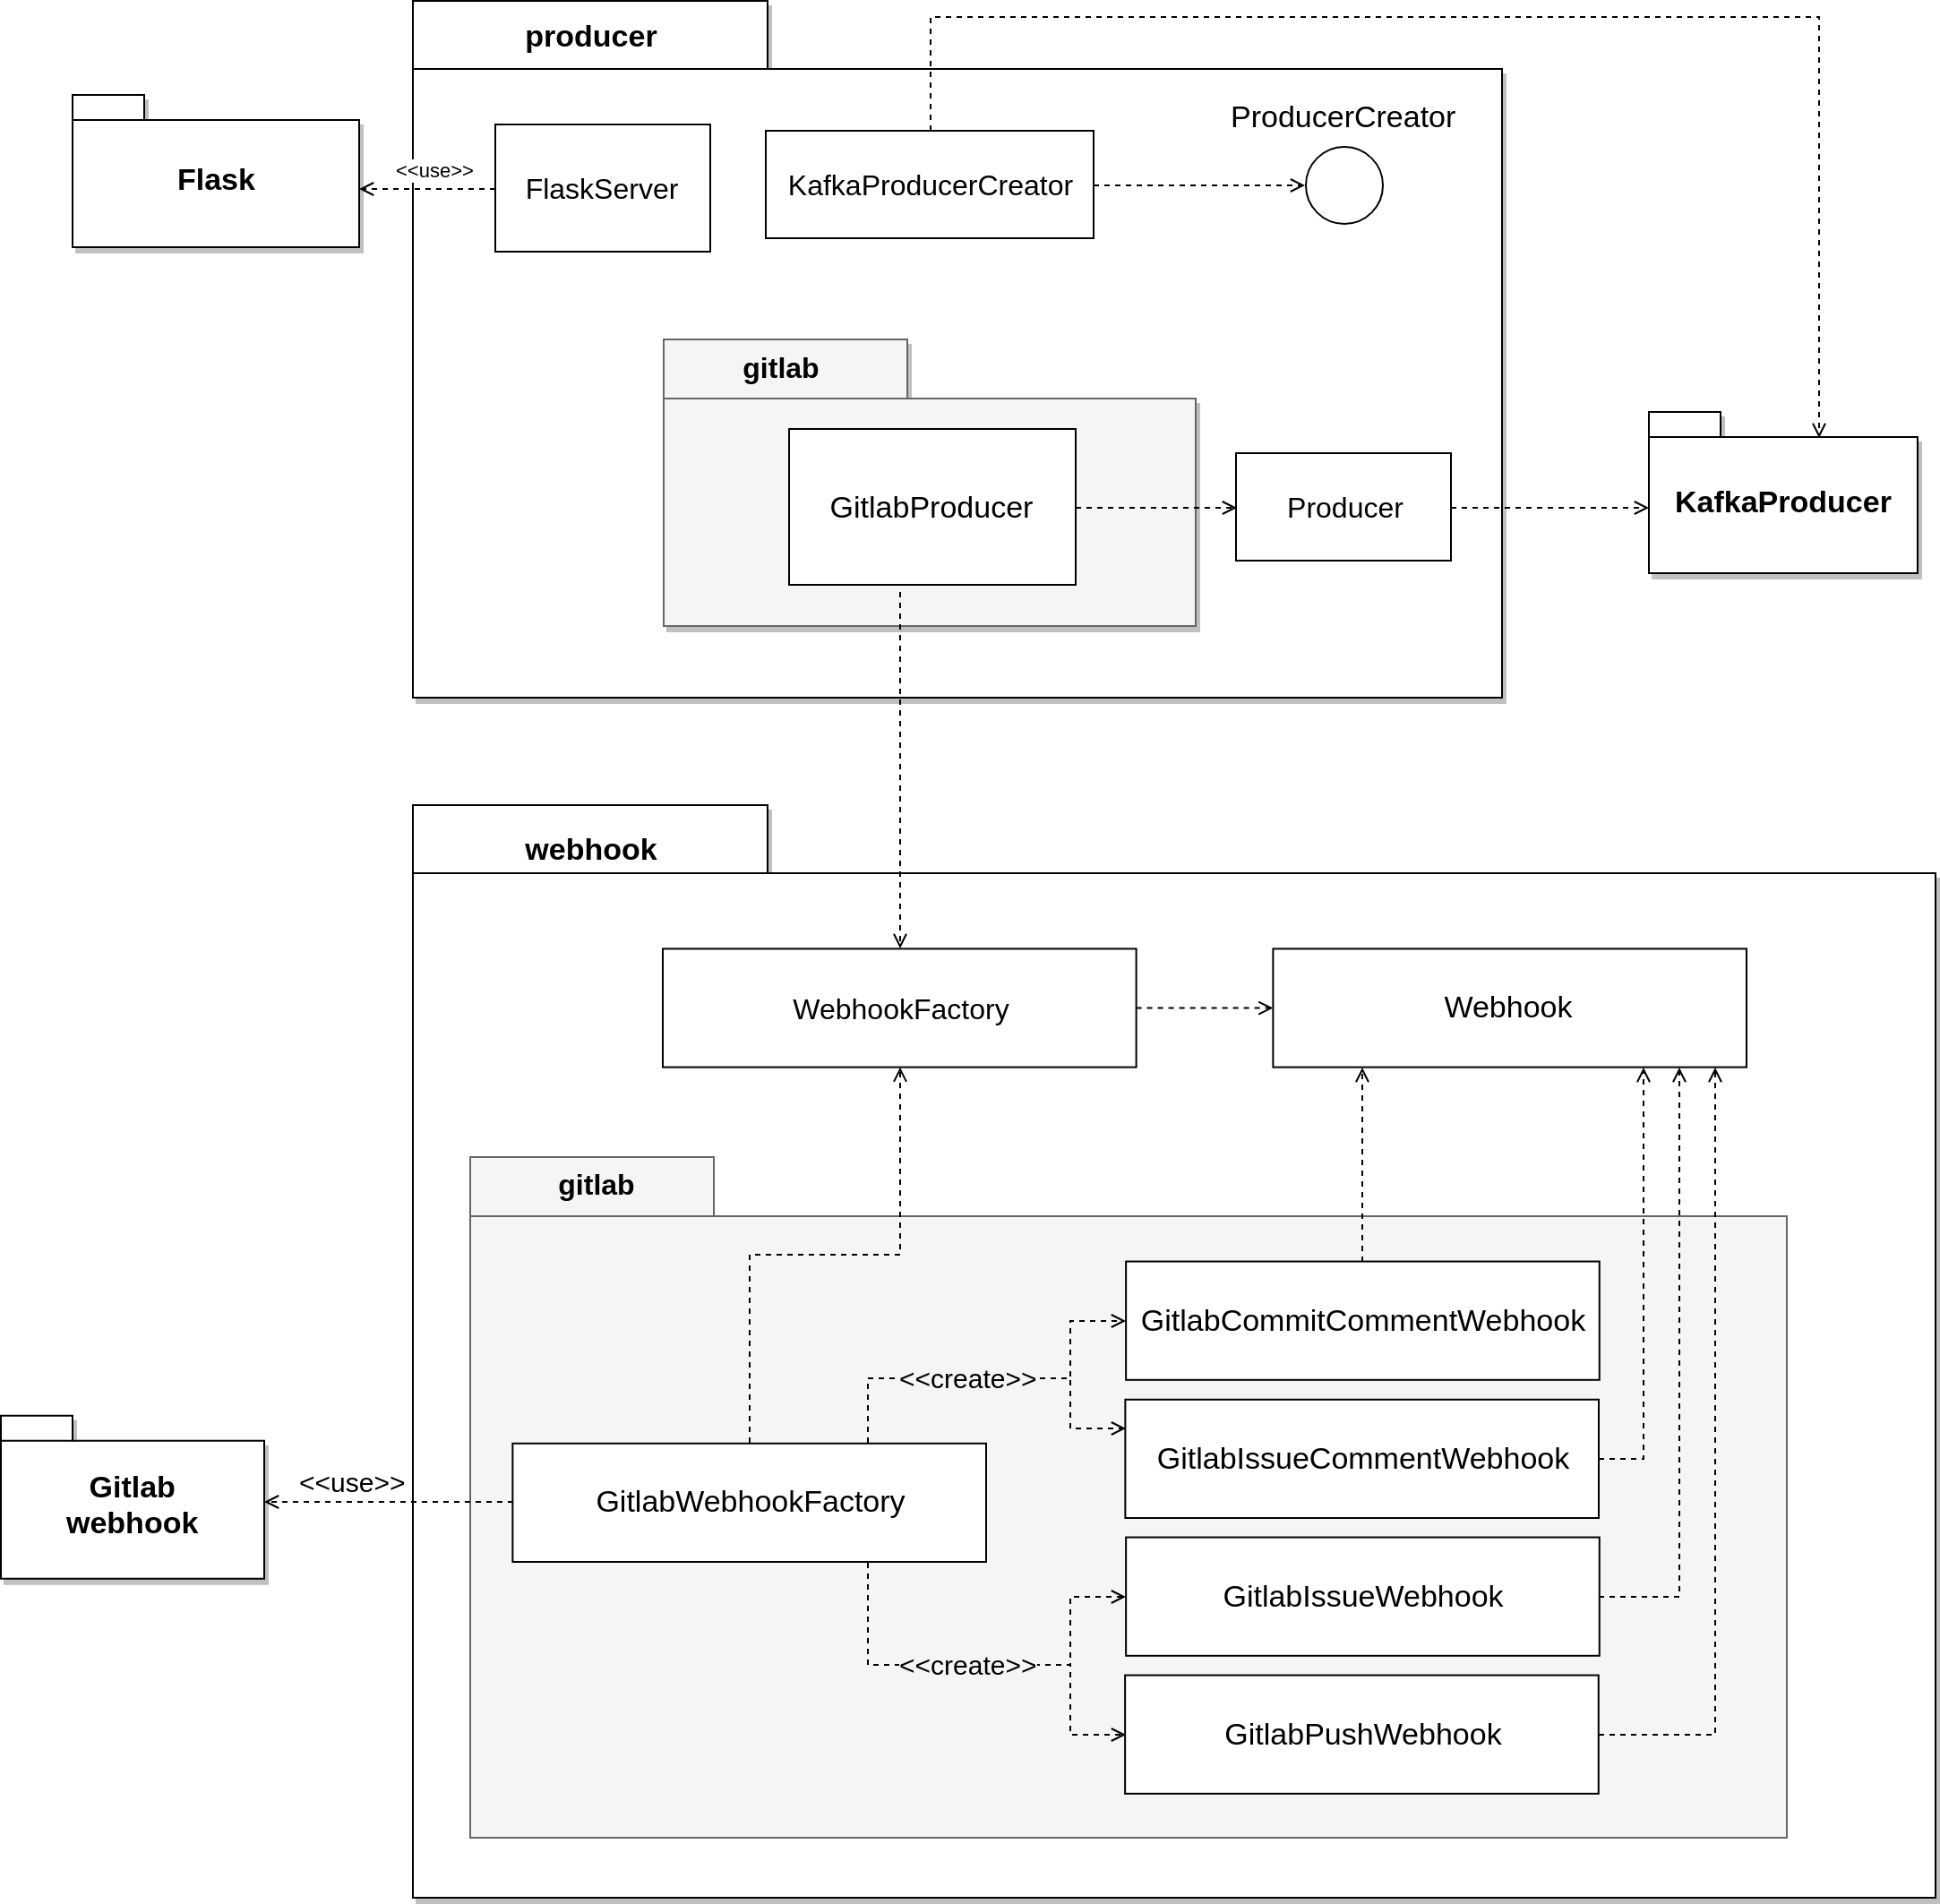
\includegraphics[width=\textwidth]{img/Package-GitLabProducer.png}\\
    \caption{Diagramma dei package di GitlabProducer}
    % \label{fig:producers}
\end{figure}


\paragraph{Diagramma delle classi}

\begin{figure}[H]
    \centering
    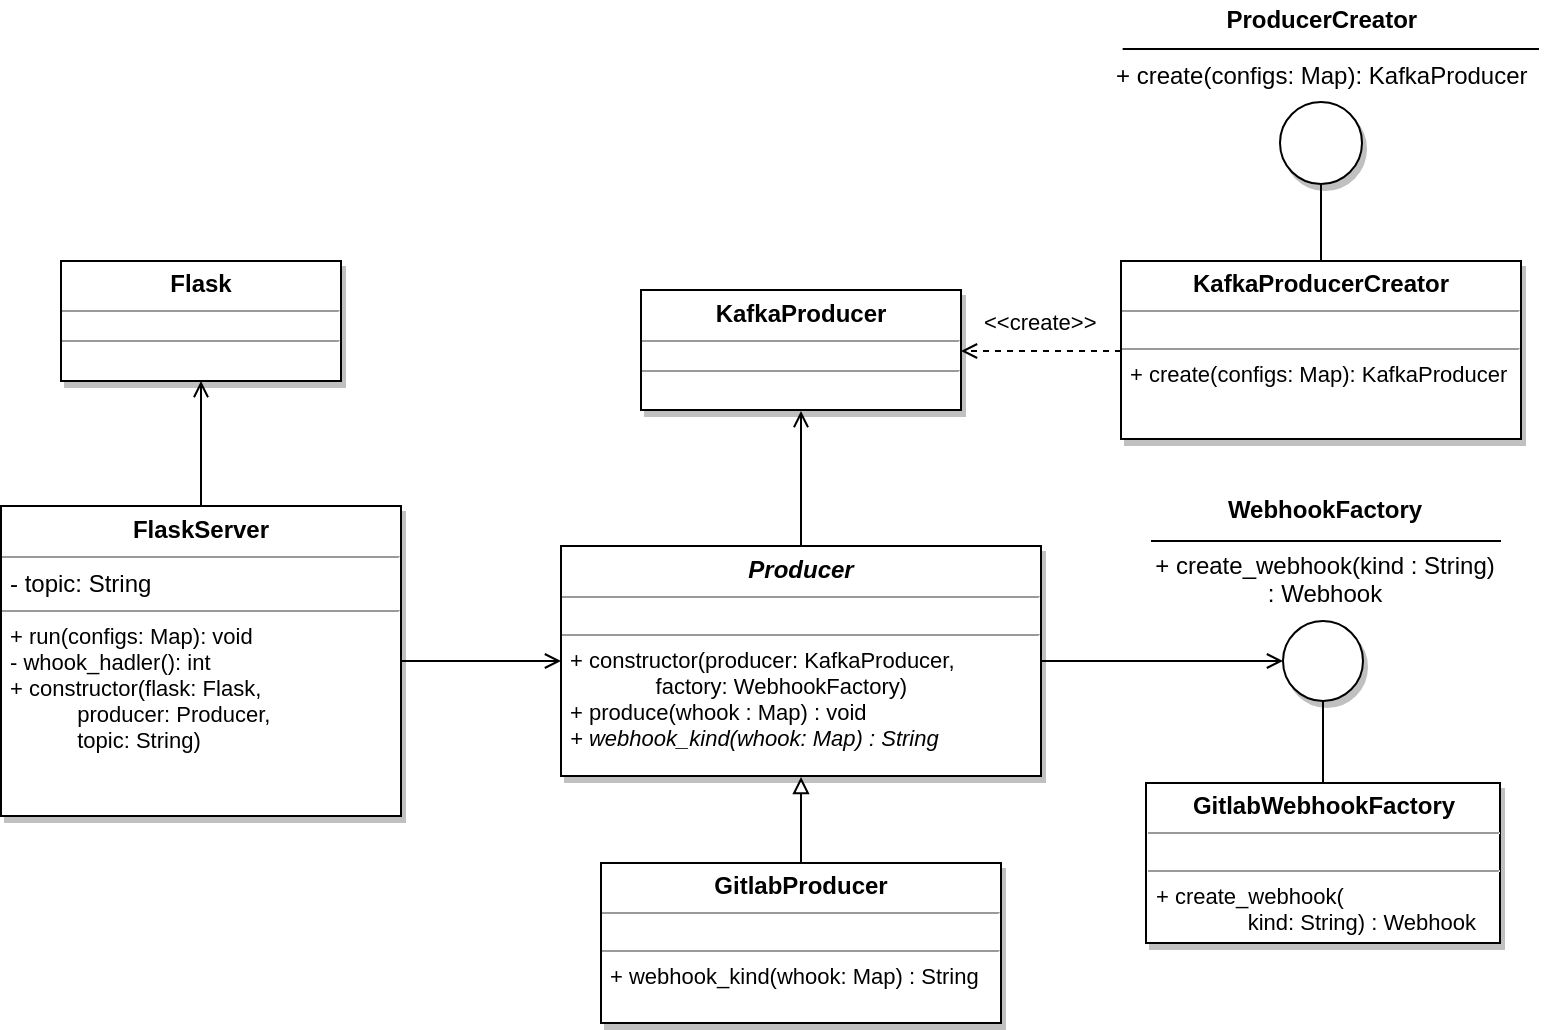
\includegraphics[width=\textwidth]{img/Producers-GitlabProducer.png}\\
    \caption{Diagramma delle classi di GitlabProducer}
    % \label{fig:producers}
\end{figure}

Abbiamo implementato per GitlabProducer 4 tipologie di \texttt{Webhook}.
Il parametro \texttt{kind} del metodo \texttt{create\_webhook(kind)} può quindi assumere 4 valori, in base al quale
\texttt{GitlabWebhookFactory} costruirà un parser di Webhook apposito:
\begin{itemize}
    \item '\texttt{issue}': verrà istanziato un \texttt{GitlabIssueWebhook}.
    \item '\texttt{push}': verrà istanziato un \texttt{GitlabPushWebhook}.
    \item '\texttt{issue-comment}': verrà istanziato un \texttt{GitlabIssueCommentWebhook}.
    \item '\texttt{commit-comment}': verrà istanziato un \texttt{GitlabCommitCommentWebhook}.
\end{itemize}

Questo è un pattern creazionale specifico: \gloss{Factory Method}.


\begin{figure}[H]
    \centering
    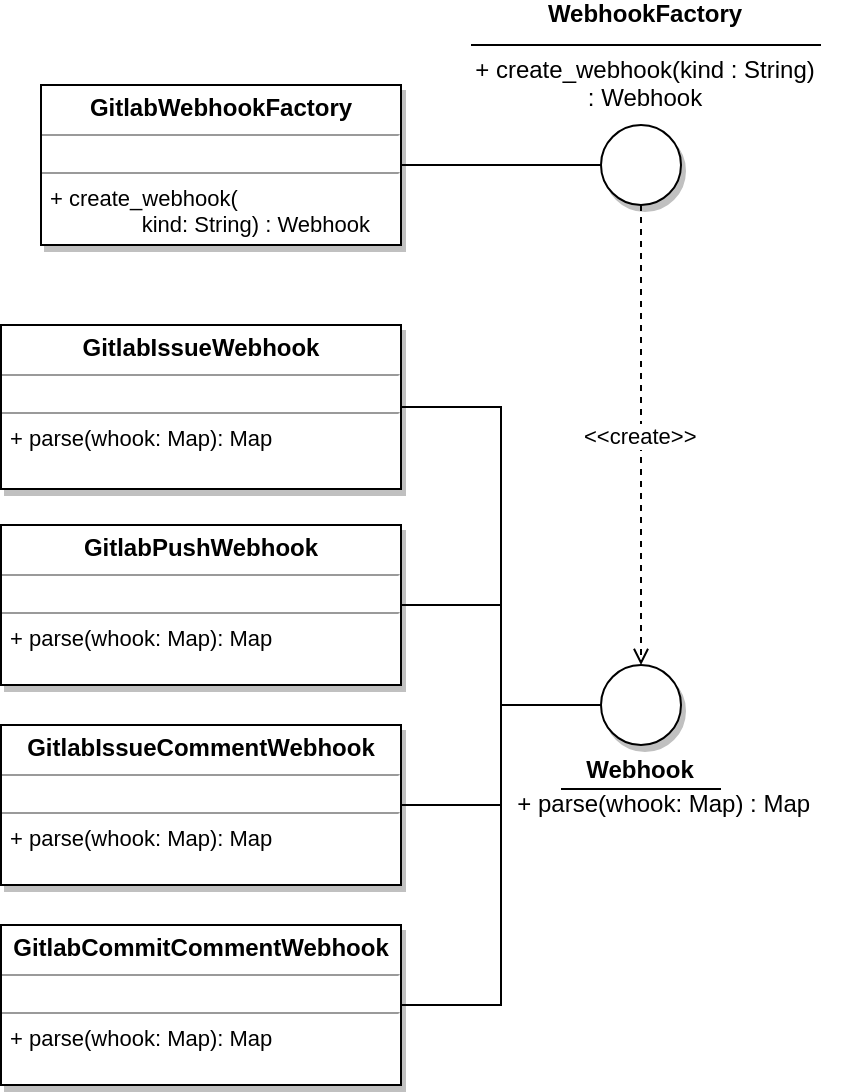
\includegraphics[width=0.6\textwidth]{img/Producers-GitlabWebhook.png}\\
    \caption{Diagramma delle classi di GitlabWebhookFactory}
    % \label{fig:producers}
\end{figure}



\subsection{Gestore Personale}
Il Gestore Personale è la componente con la logica più complessa del sistema Butterfly. Esso ha un proprio KafkaProducer e KafkaConsumer
che si occupano rispettivamente di ricevere i messaggi da Kafka e reinserirli nelle code relative ai Consumer finali. Per stabilire il destinatario e il Consumer finale appropriato, il Client del Gestore Personale interroga MongoDB per ottenere per selezionare i giorni di indisponibilità, la priorità dei progetti e la piattaforma di messaggistica sul
quale ricevere la notifica per ogni utente. Tutte queste informazioni vengono inserite in MongoDB attraverso la View. \par
Questa prima parte riguarda la sezione del gestore personale che va a interfacciarsi con l’utente adottando un’architettura MVC pull model.
La View è pertanto totalmente passiva e l’unica cosa che fa è inoltrare i comandi ricevuti dall’utente al Controller.

\subsubsection{Diagramma dei package}

\begin{figure}[H]
    \centering
    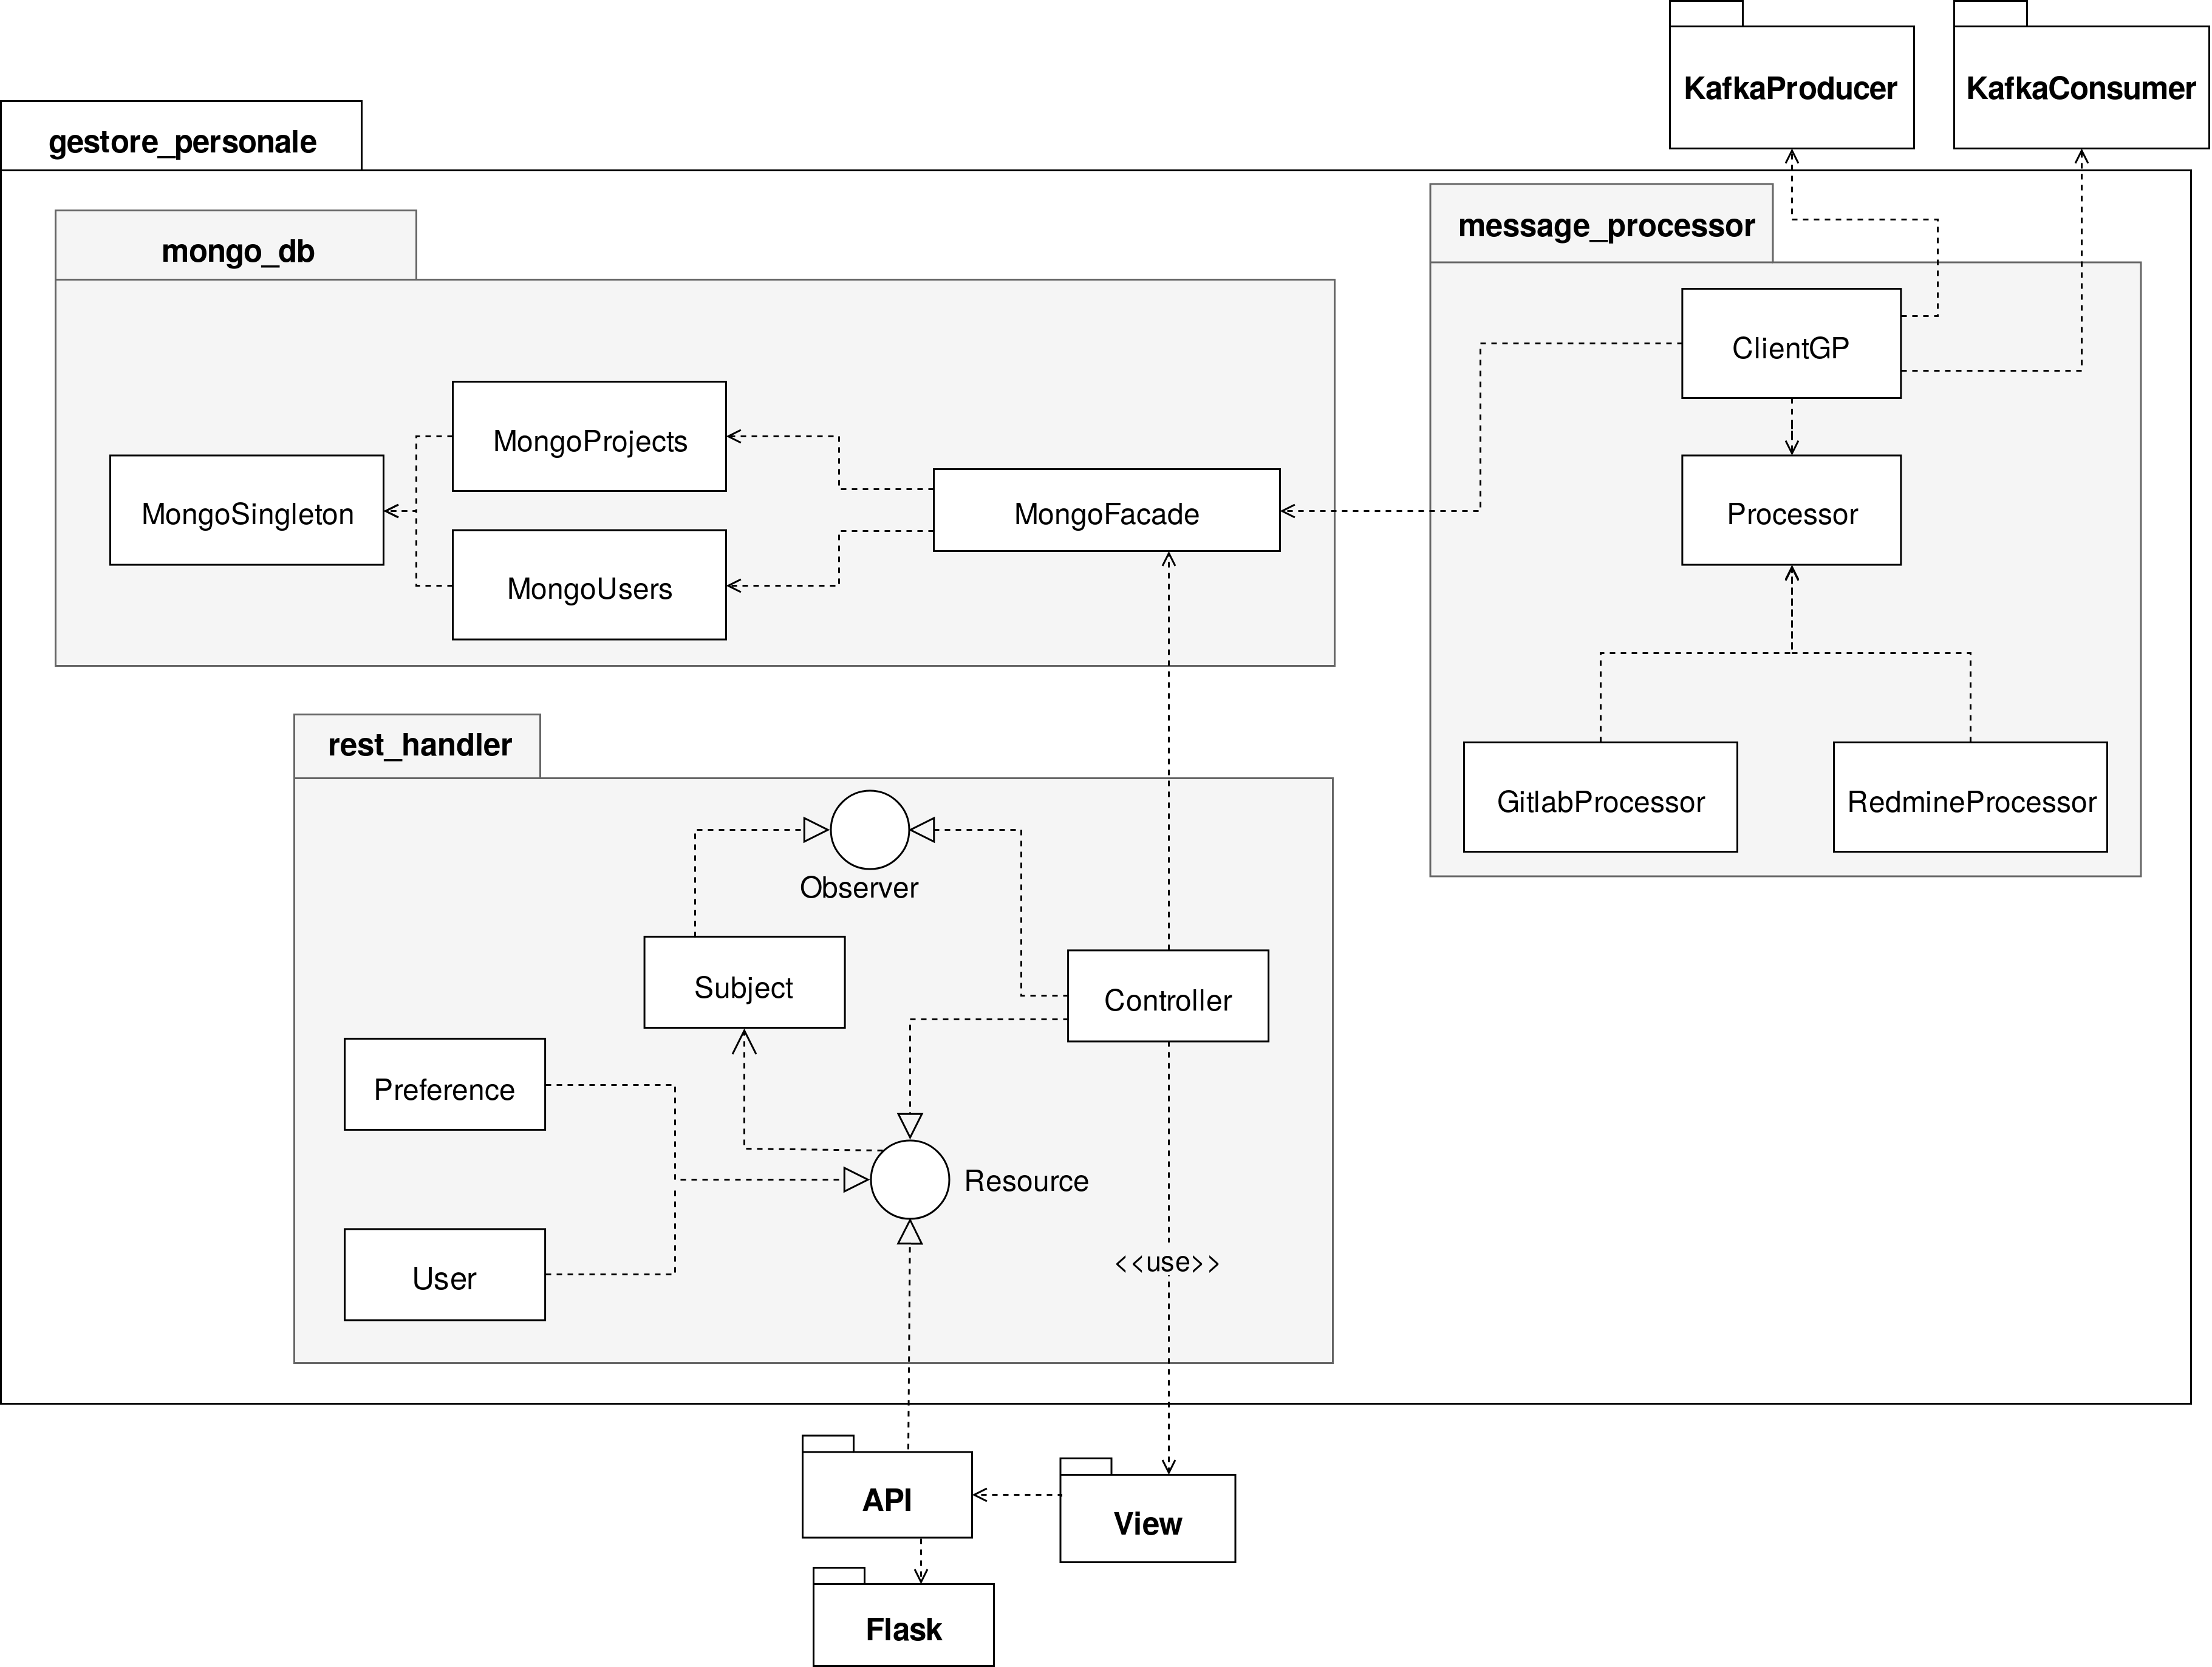
\includegraphics[width=\textwidth]{img/Package-GestorePersonale.png}\\
    \caption{Diagramma dei package del Gestore Personale}
    % \label{fig:GP-Processor}
\end{figure}

\subsubsection{Mongo}
Model dell'MVC

    \paragraph{Diagramma delle classi}
    Qua viene mostrato come il Gestore Personale si interfaccia con \gloss{MongoDB}, ovvero MongoUser e MongoProject. Sono suddivisi in base alla risorsa di interesse.

    \begin{figure}[H]
        \centering
        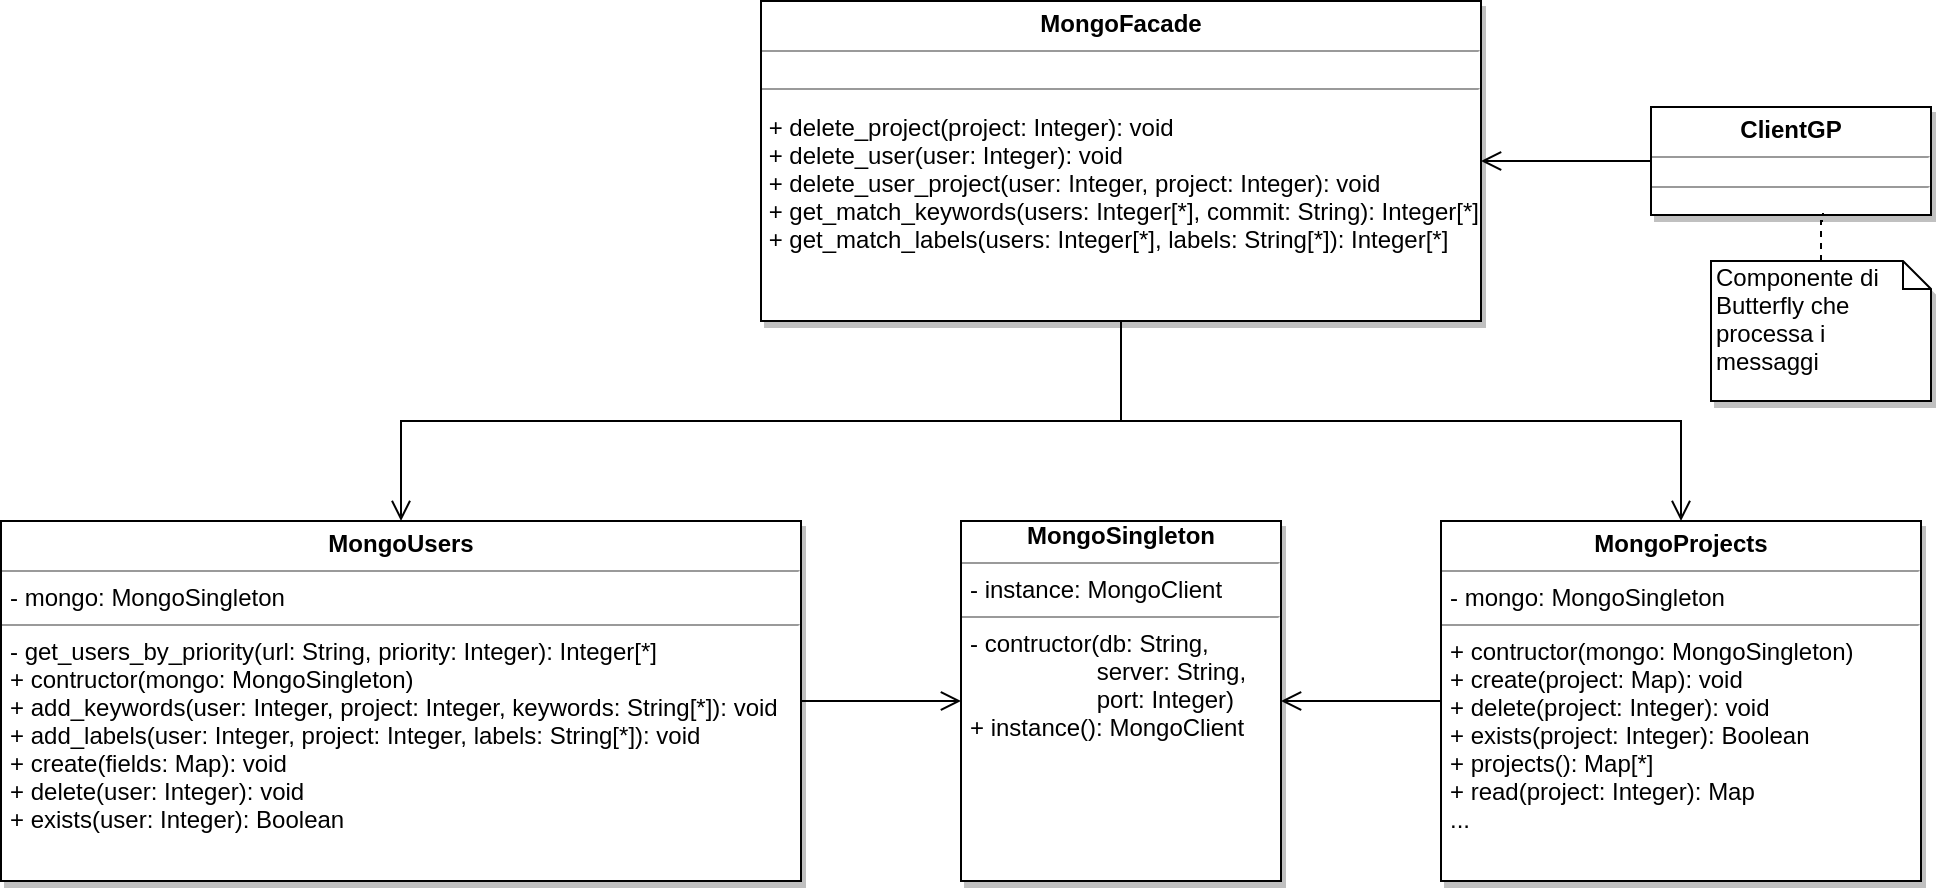
\includegraphics[width=\textwidth]{img/GP-Mongo.png}\\
        \caption{Interazione con MongoDB del Gestore Personale}
        \label{fig:GP-Mongo}
    \end{figure}


\subsubsection{Controller e View}
Il Controller del Gestore Personale serve per collegare la componente del Model con la componente View.
Una volta istanziati il server Flask, l'api REST e MongoDB vengono passati al Controller che resta in ascolto.\par
Quando arriva una richiesta dall'api REST o dalla View, il Controller esegue le dovute operazioni su MongoDB e restituisce una risposta alla vista di provenienza, in formato JSON se si tratta dell'api REST o in formato HTML se si tratta della view consultabile da browser Web.


    \paragraph{Diagramma delle classi}

    \begin{figure}[H]
        \centering
        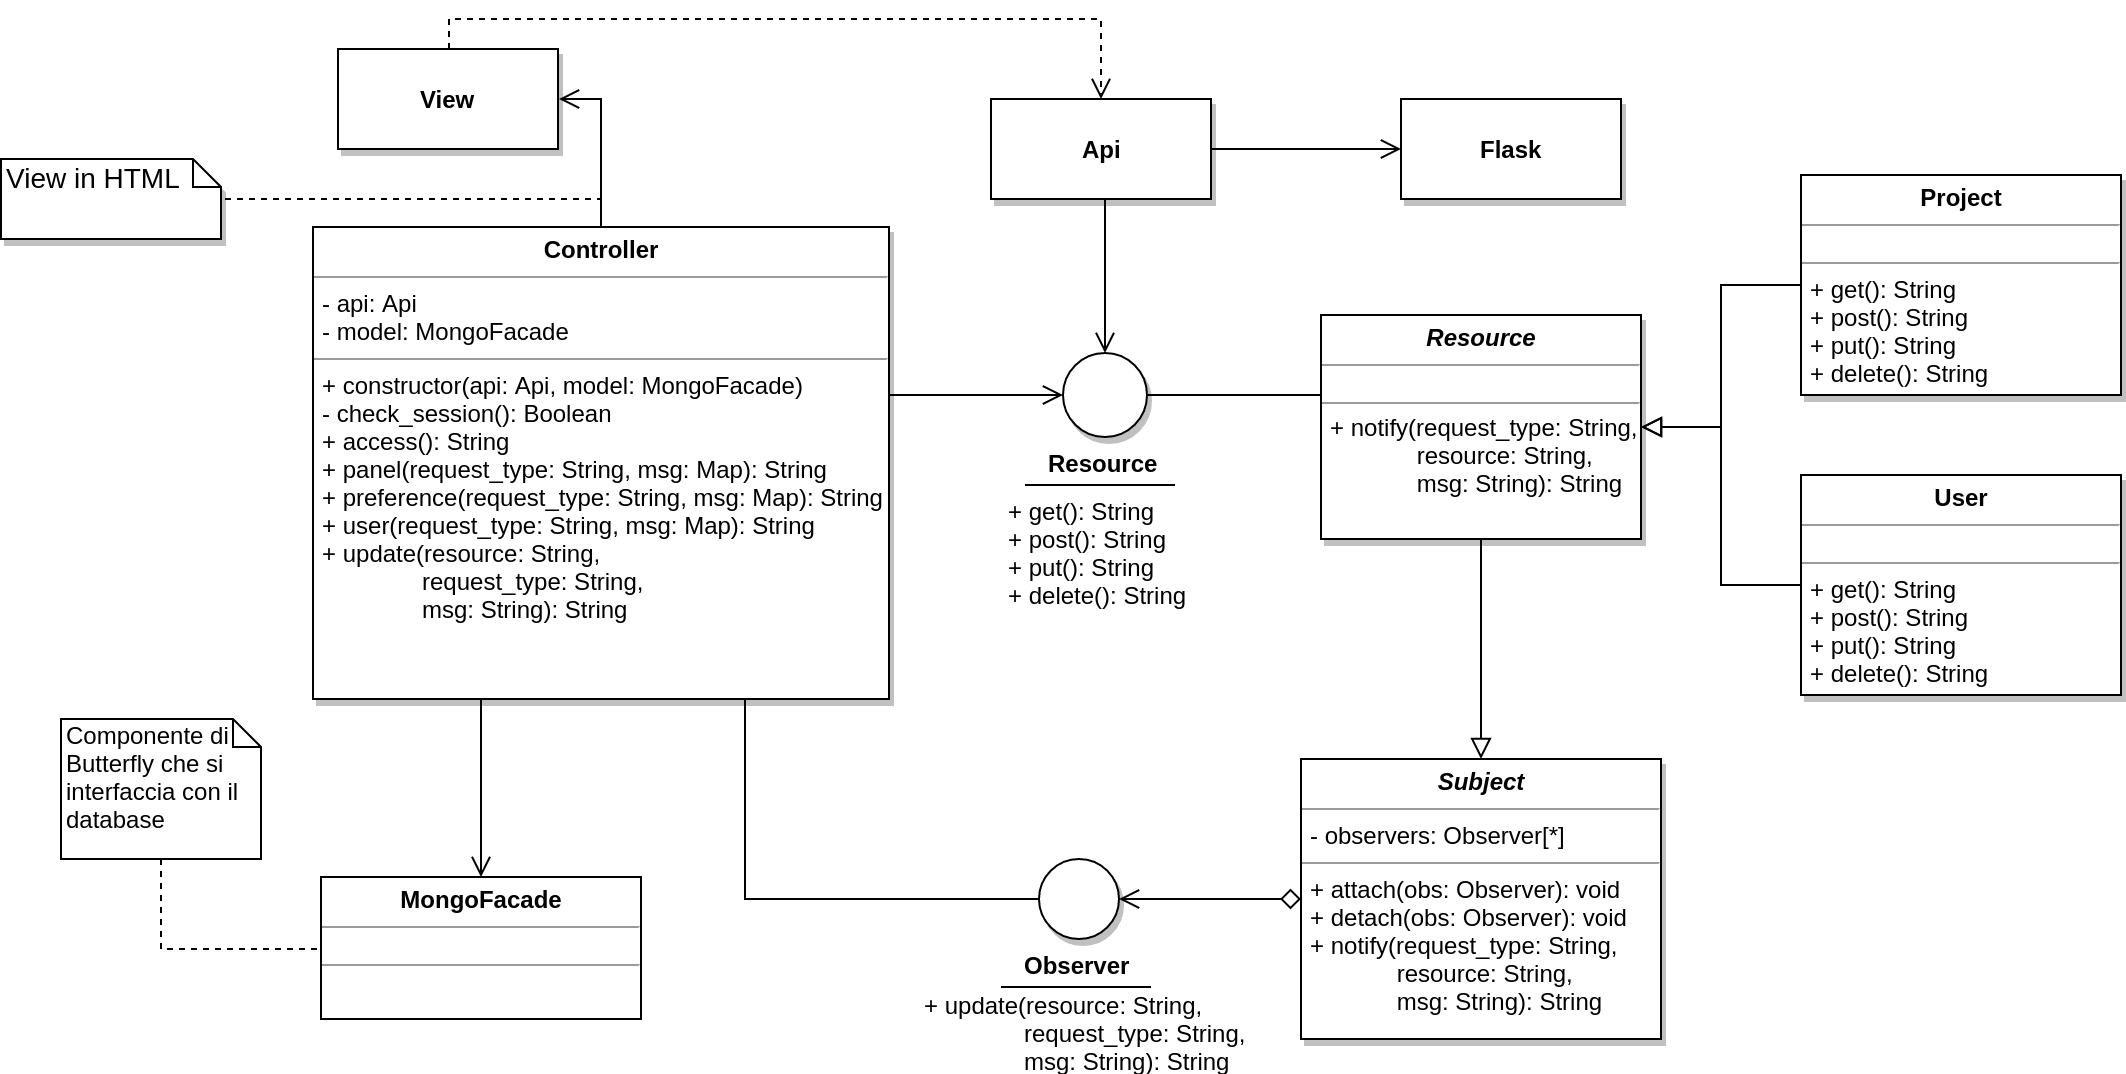
\includegraphics[width=\textwidth]{img/GP-View.png}\\
        \caption{Logica del Controller del Gestore Personale}
        \label{fig:GP-View}
    \end{figure}



%\newpage
\subsubsection{Client}
Il suo compito è quello di recuperare i messaggi inseriti in Kafka dai Producer GitLab e Redmine attraverso un Consumer fittizio, analizzare il messaggio, associargli il destinatario corretto e inserirlo nella coda di Kafka appropriata (di Telegram o Email) attraverso un Producer fittizio.

Per analizzare il messaggio il Client opera in questo modo:

\begin{figure}[H]
    \centering
    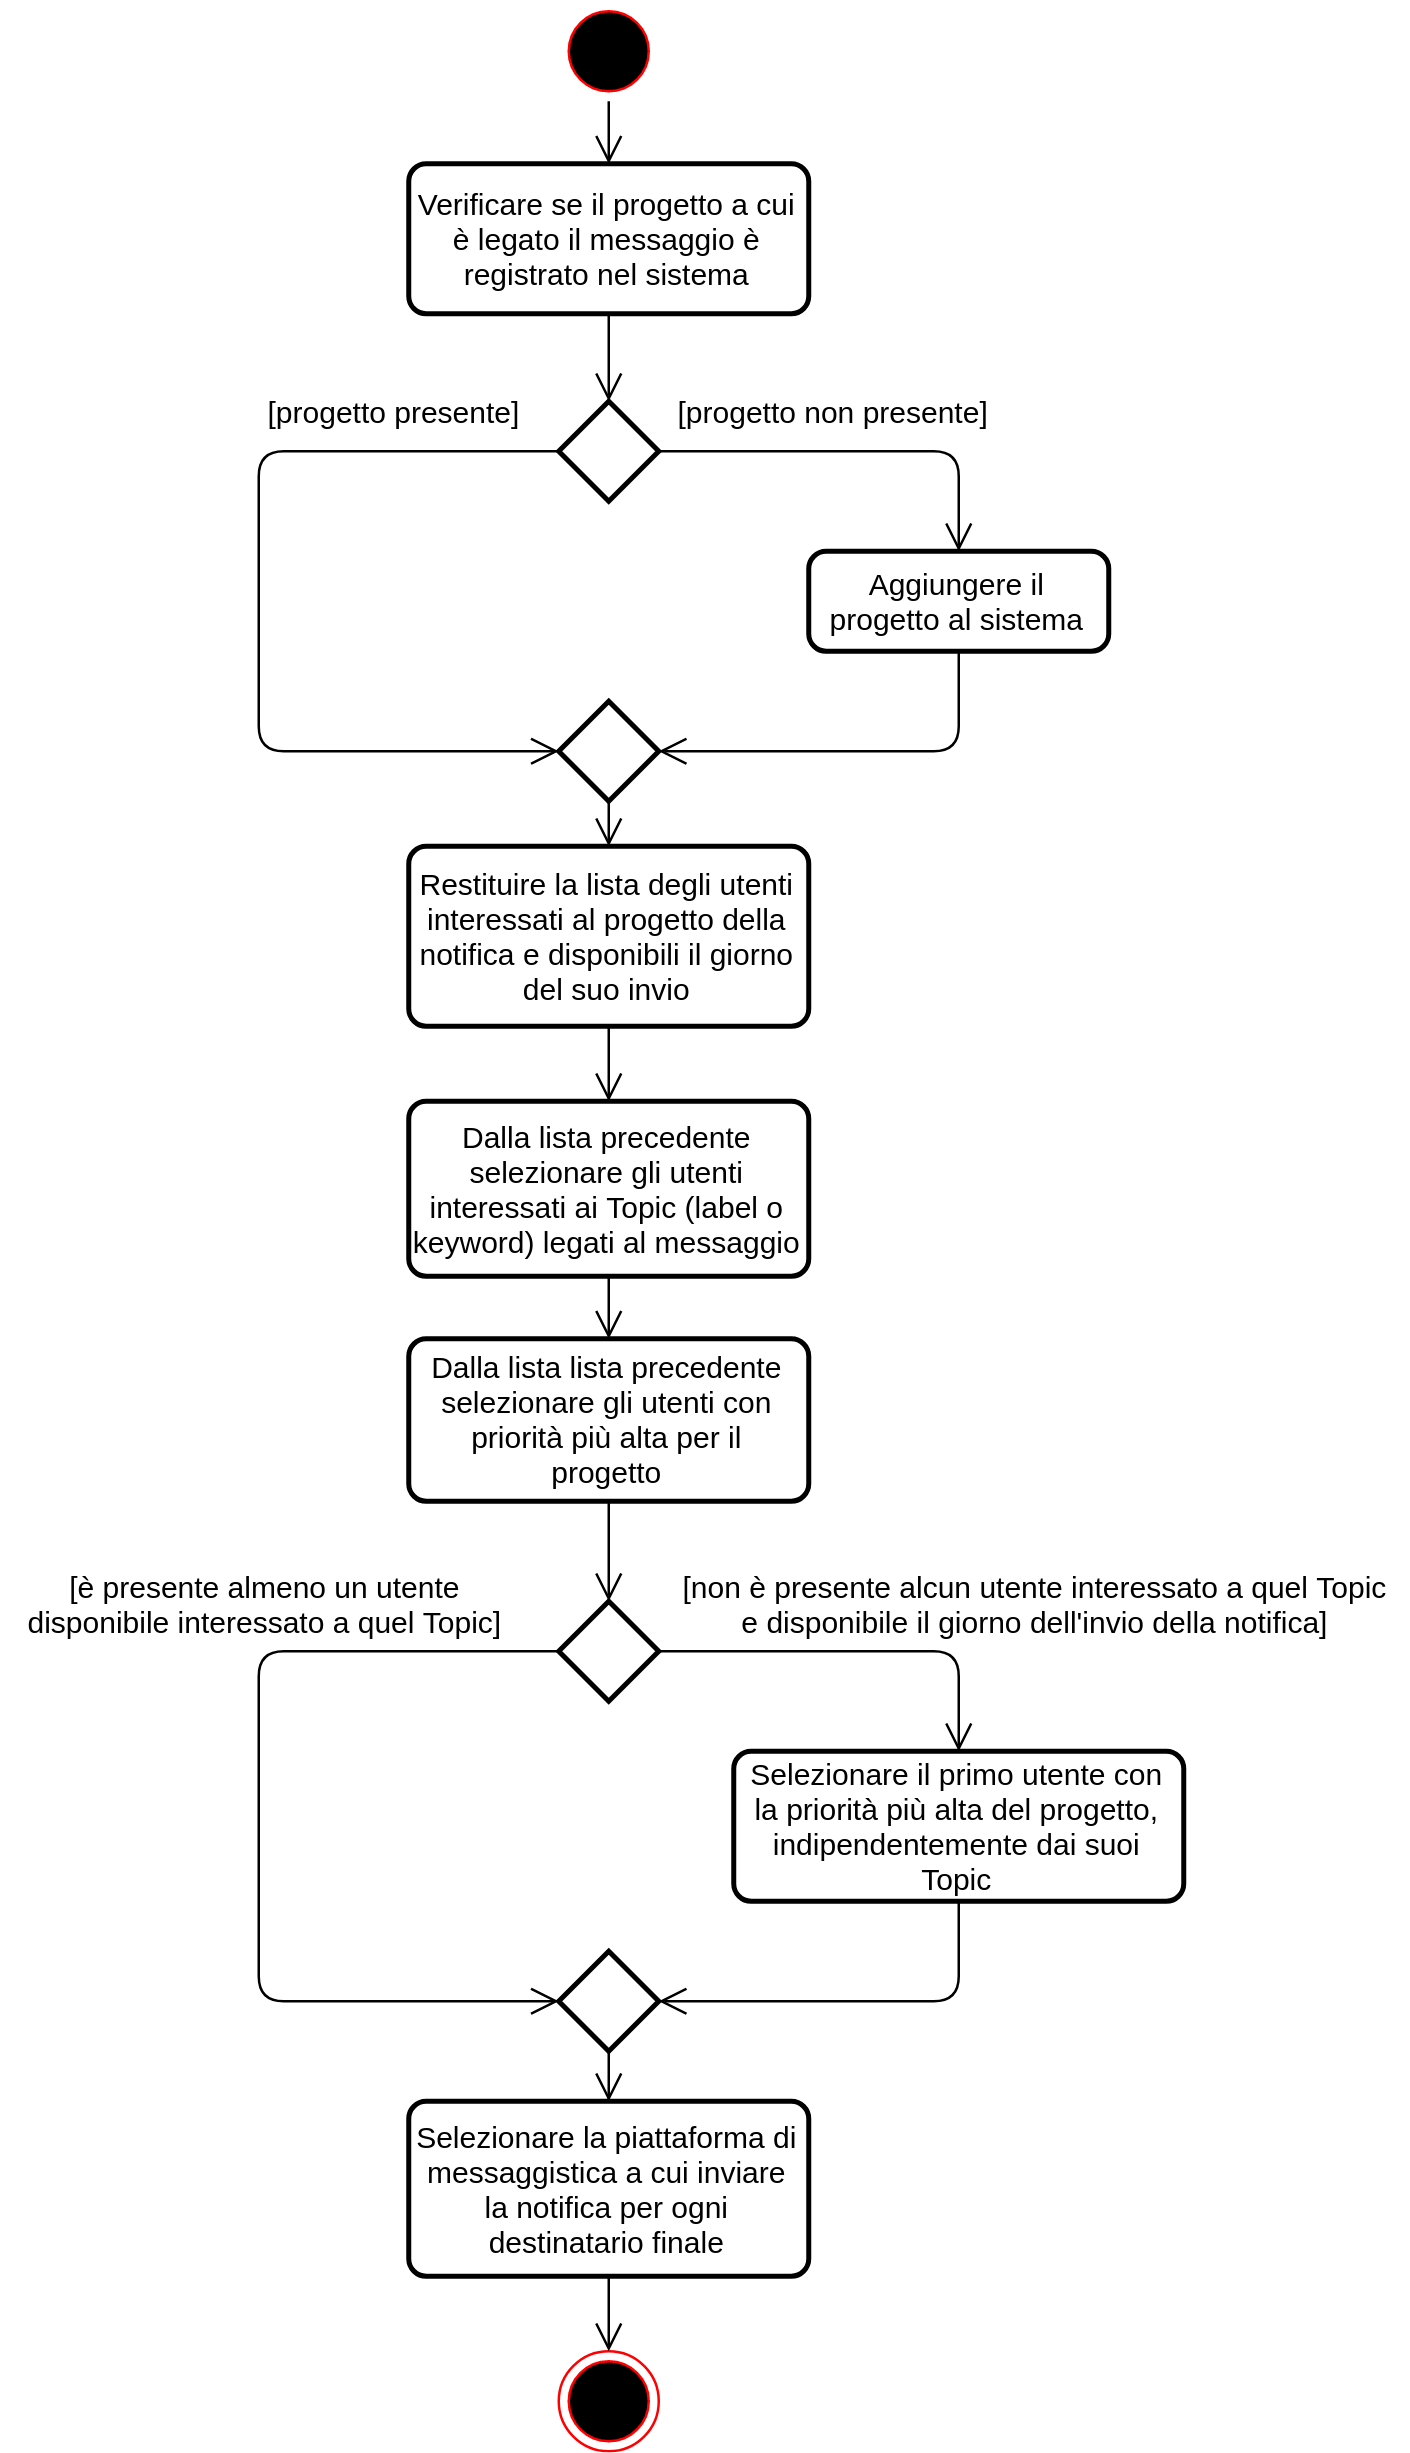
\includegraphics[width=0.69\textwidth]{img/Client_attivita.png}\\
    \caption{Diagramma di attività del Client}
    % \label{fig:GP-Processor}
\end{figure}

    \paragraph{Diagramma delle classi}
    .. viene mostrato come il Gestore Personale si interfaccia con Kafka, questa riguarda il core del Gestore Personale, si occupa di processare
    i messaggi.

    \begin{figure}[H]
        \centering
        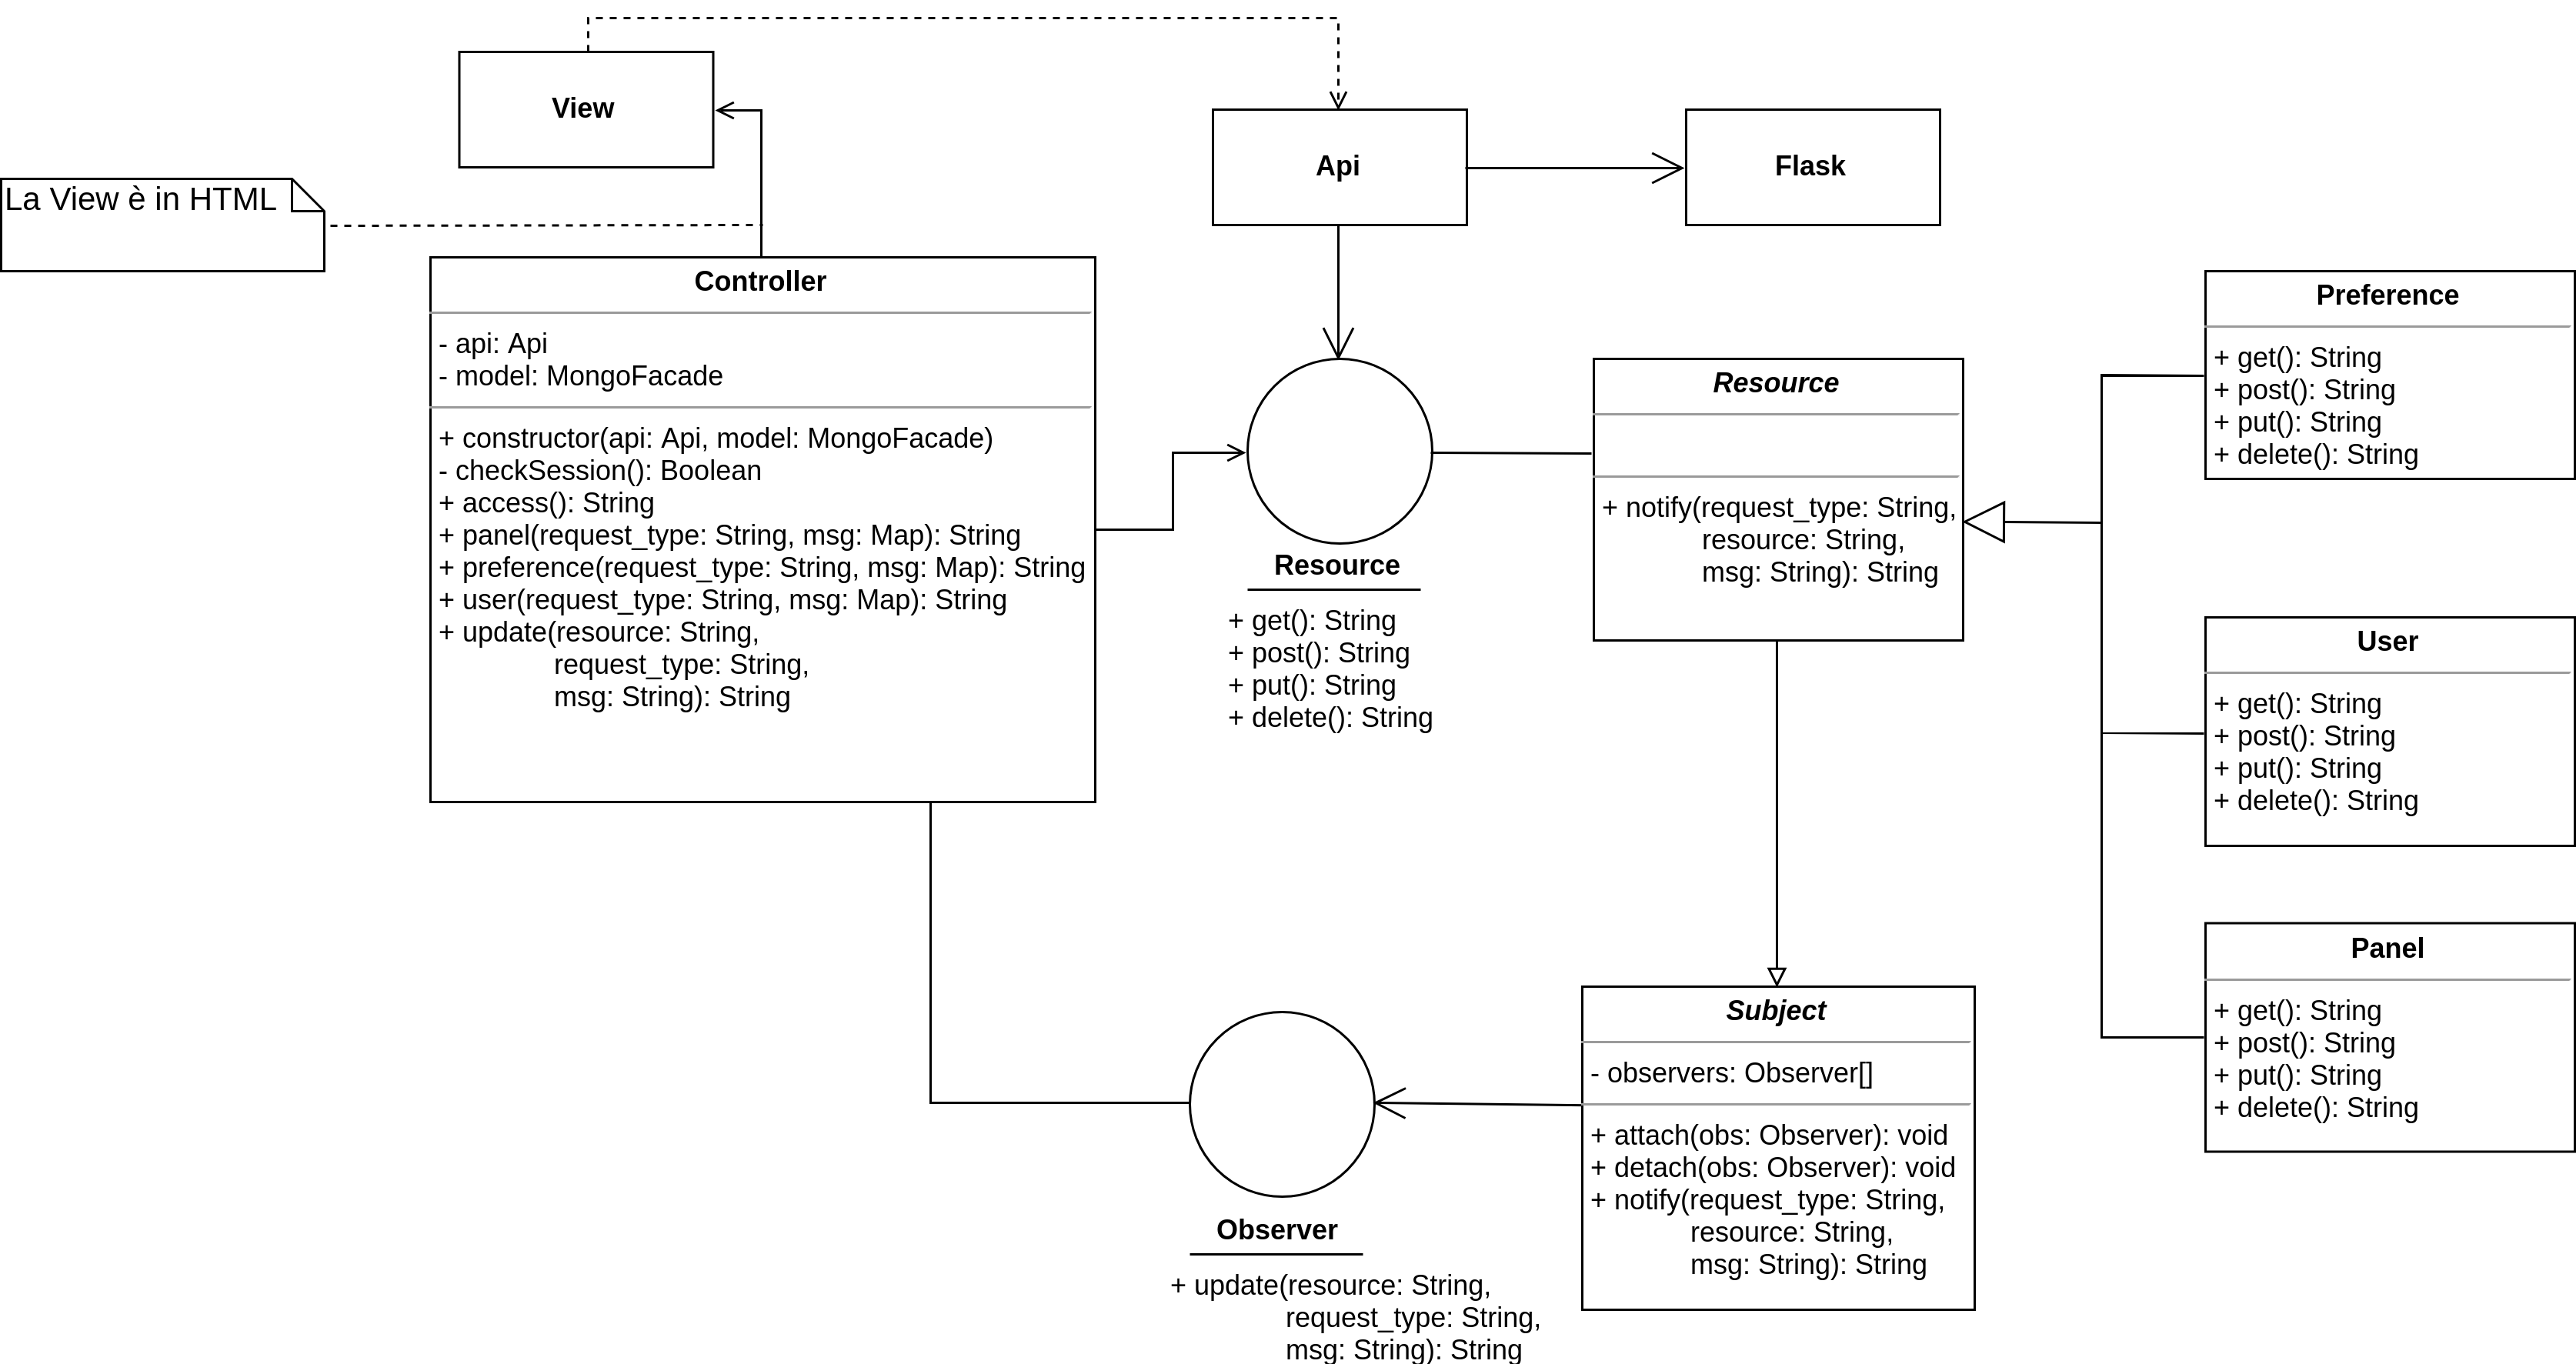
\includegraphics[width=\textwidth]{img/GP-Processor.png}\\
        \caption{Message processor del Gestore Personale}
        \label{fig:GP-Processor}
    \end{figure}




\subsection{Consumers}
Il Consumer è la componente finale del sistema \progetto. Esso resta in ascolto della sua coda specifica di Kafka per applicativo (e.g. telegram, email).
Si occupa di inoltrare il messaggio al destinatario finale.

Al momento della stesura di questo manuale, i Consumer implementati sono due:

\begin{itemize}
    \item TelegramConsumer
    \item EmailConsumer
\end{itemize}

L'algoritmo di ascolto dei messaggi è identico per ogni Consumer: come per i Producer, abbiamo utilizzato
Template Method per l'implementazione di \texttt{listen()}.
Le classi concrete avranno esclusivamente il compito di implementare il metodo \texttt{send()}, il quale invierà il messaggio
al destinatario finale tramite le API dell'applicativo su cui il Consumer è basato.


\subsubsection{TelegramConsumer}

\paragraph{Diagramma dei package}

Il TelegramConsumer ha 2 dipendenze esterne:
\begin{itemize}
    \item \texttt{KafkaConsumer} dalla libreria esterna \texttt{kafka-python}: offre le funzionalità di ascolto
        di una o più code specifiche. È costruito su di esso un adapter, per adattare KafkaConsumer alle funzionalità
        di \texttt{Consumer}.
    \item Package \texttt{requests}: effettua le richieste POST e poter inviare i messaggi tramite l'API di Telegram
        al destinatario finale.
\end{itemize}

\begin{figure}[H]
    \centering
    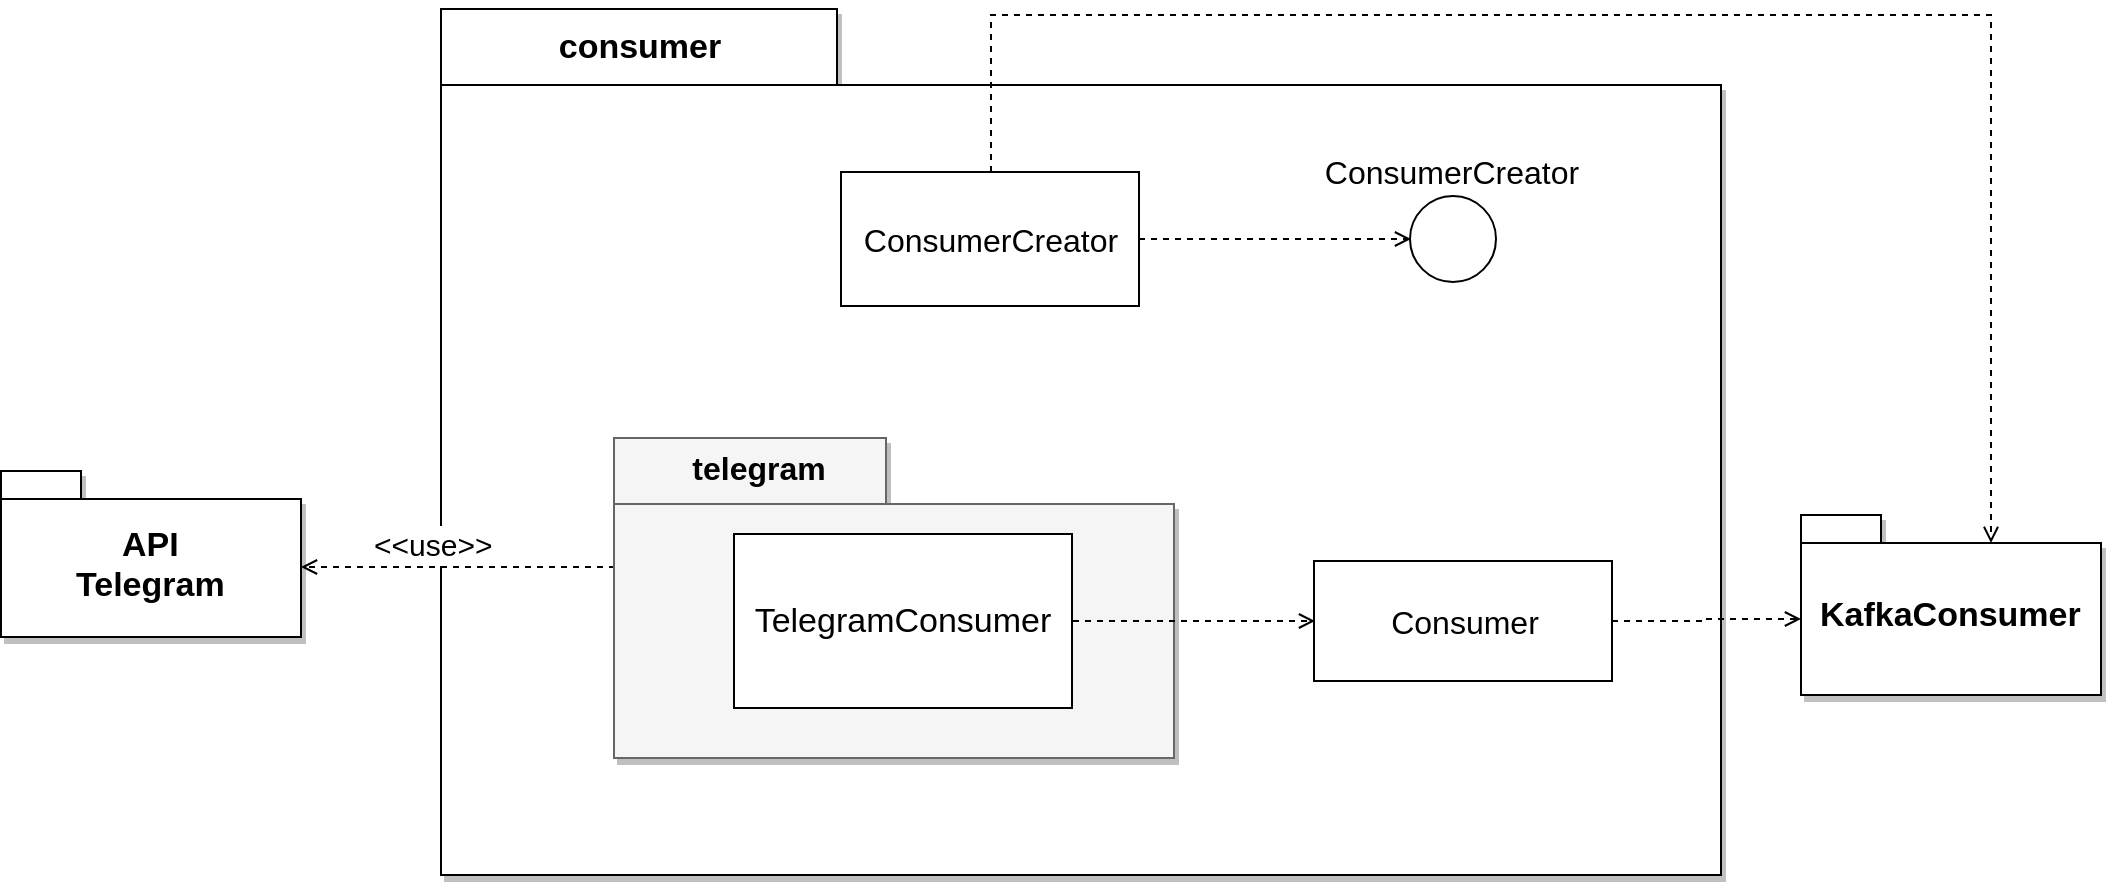
\includegraphics[width=\textwidth]{img/Package-TelegramConsumer.png}\\
    \caption{Diagramma dei package di TelegramConsumer}
    % \label{fig:GP-Kafka}
\end{figure}

\paragraph{Diagramma delle classi}

Il metodo \texttt{format()} costruisce il testo del messaggio finale utilizzando il formato \gloss{markdown} specifico per Telegram.

\begin{figure}[H]
    \centering
    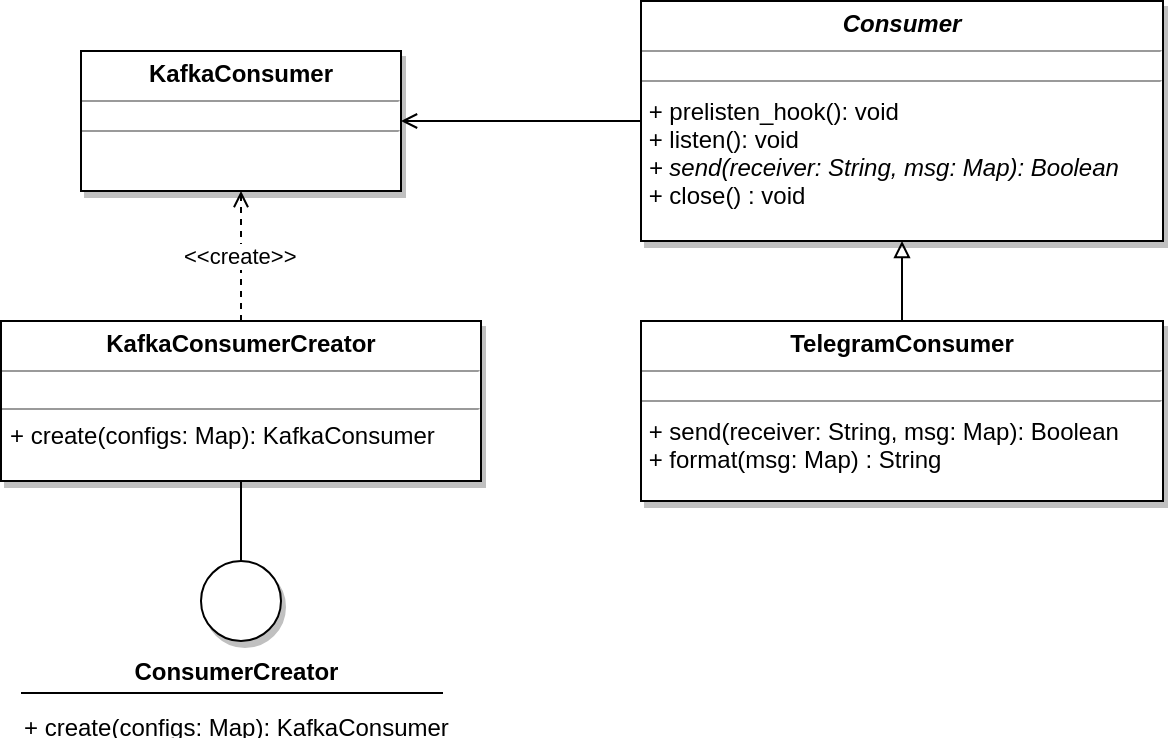
\includegraphics[width=0.8\textwidth]{img/Consumers-TelegramConsumer.png}\\
    \caption{Diagramma delle classi di TelegramConsumer}
    % \label{fig:GP-Kafka}
\end{figure}


\subsubsection{EmailConsumer}

\paragraph{Diagramma dei package}

L'EmailConsumer ha 2 dipendenze esterne:
\begin{itemize}
    \item \texttt{KafkaConsumer} della libreria esterna \texttt{kafka-python}: offre le funzionalità di ascolto dei messaggi
        proveniente da una o più code specifiche. È costruito su di esso un adapter, per adattare le funzionalità di KafkaConsumer a
        \texttt{Consumer}.
    \item \texttt{SMTP} della libreria esterna \texttt{smtplib}: server e-mail che, dopo aver effettuato il login,
        invia al destinatario una mail contenente il messaggio finale.
\end{itemize}

\begin{figure}[H]
    \centering
    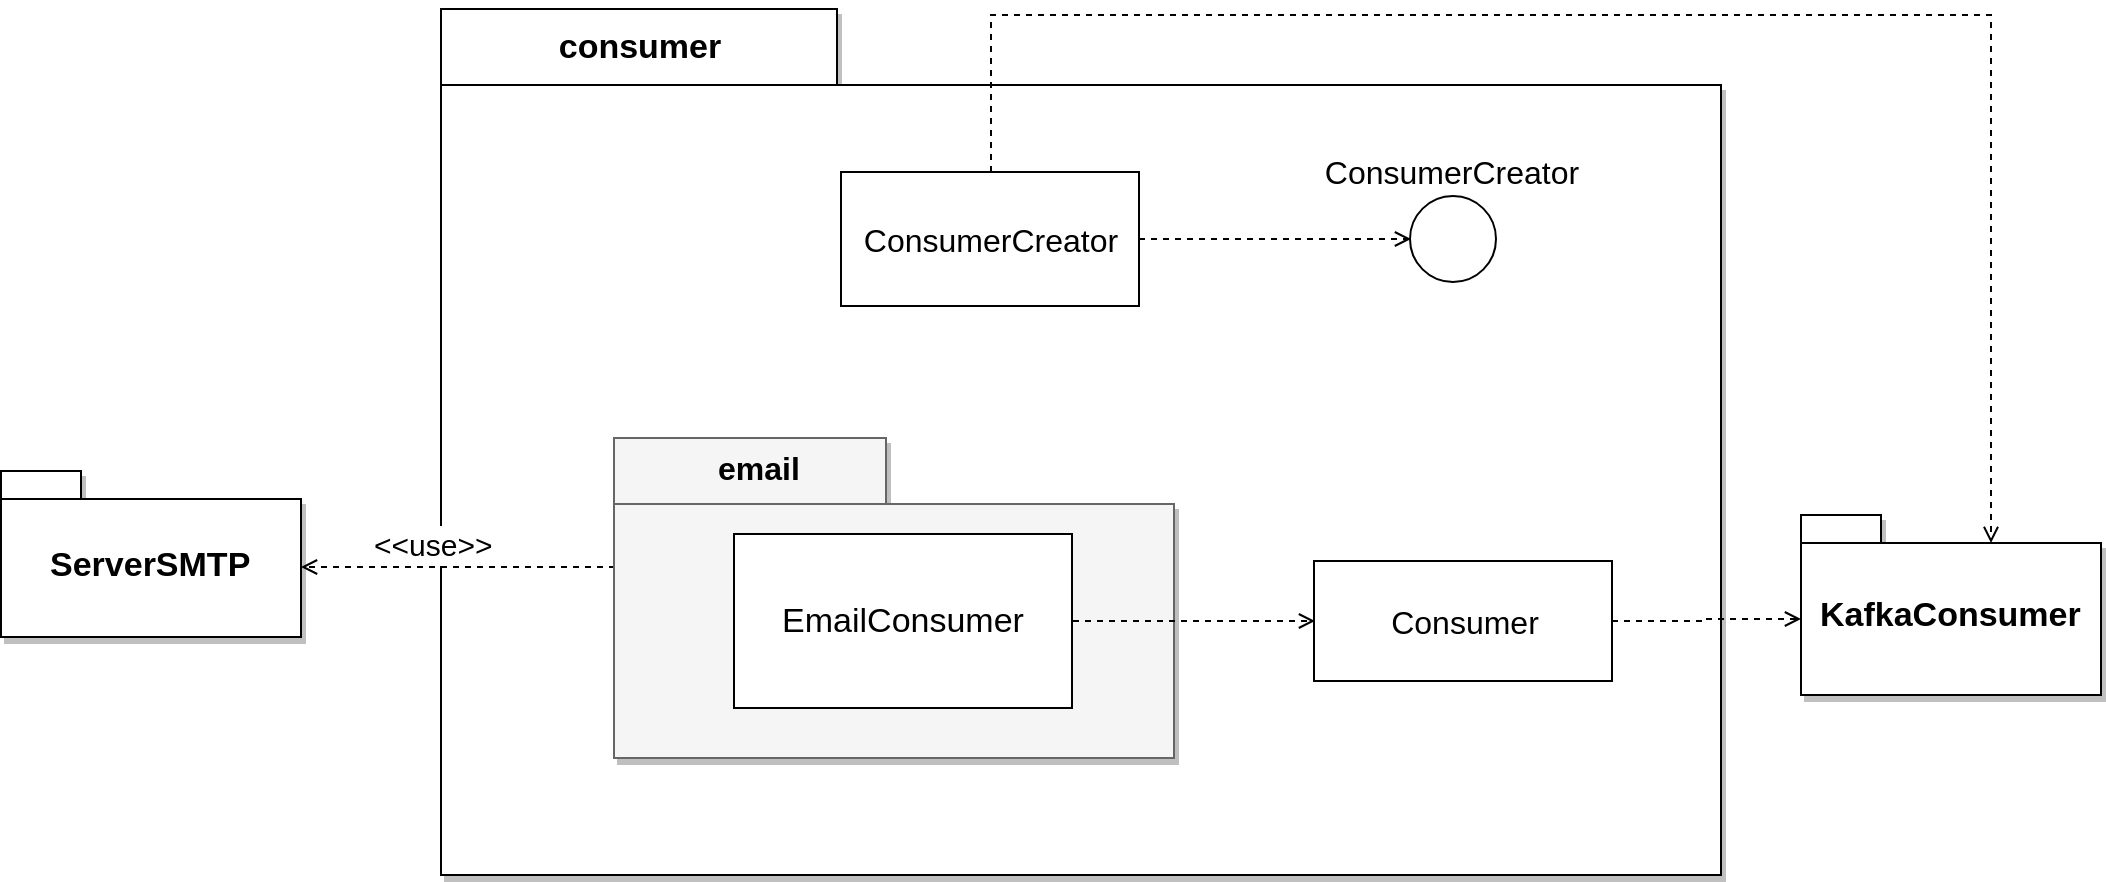
\includegraphics[width=\textwidth]{img/Package-EmailConsumer.png}\\
    \caption{Diagramma dei package di EmailConsumer}
\end{figure}


\paragraph{Diagramma delle classi}

\begin{itemize}
    \item Il metodo \texttt{format\_html()} costruisce il testo del messaggio finale in formato HTML
    \item Il metodo \texttt{format()} costruisce il testo per il messaggio senza i tag HTML, in caso il client mail del ricevente non sia in grado
        di interpretare tale linguaggio
\end{itemize}

\begin{figure}[H]
    \centering
    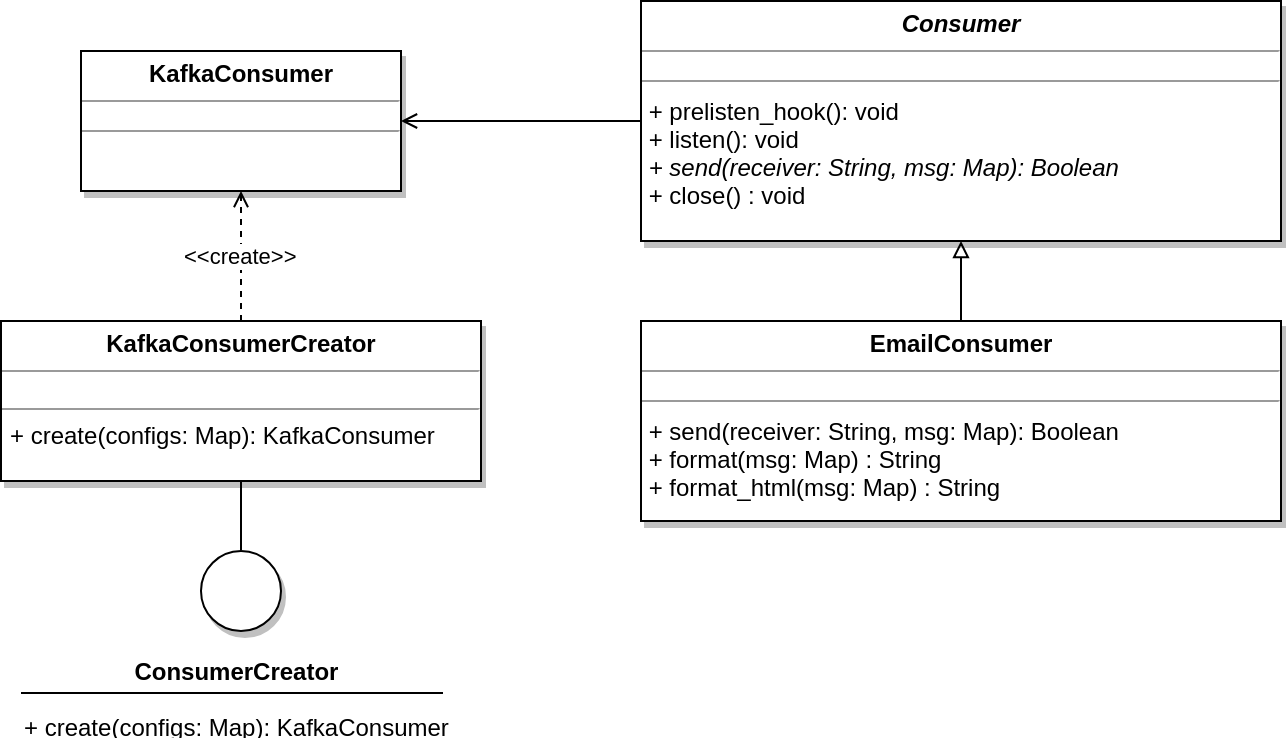
\includegraphics[width=0.8\textwidth]{img/Consumers-EmailConsumer.png}\\
    \caption{Diagramma delle classi di EmailConsumer}
    % \label{fig:GP-Kafka}
\end{figure}


\subsection{Impostazioni dei vari componenti}

Per fare in modo che tutti i componenti vengano istanziati con i determinati parametri che permettano la giusta comunicazione tra le componenti,
ci sono dei file di configurazioni che contengono per esempio il token del bot Telegram, l'email e la password per accedere al server Email. Queste configurazioni
sono contenute nei file \texttt{``config.json''} contenuto nelle cartelle producer e consumer.

\subsection{Interazione tra i componenti}

\progetto\ vedendola ad alto livello si identificano 6 componenti. Redmine e GitLab per comunicare con i relativi Producer utilizzano dei webhook in formato JSON,
mettendosi in ascolto su determinate porte utilizzando il webserver Flask. Per quanto riguarda la comunicazione tra i Producer e Kafka utilizziamo delle istanze
di KafkaProucer. Per far comunicare Kafka con i vari Consumer utilizziamo istanze di KafkaConsumer. Nell'ultimo passo, quello che riguarda i Consumer e le applicazioni finali, quali Telegram e Email, usiamo le API messe a disposizione dagli applicativi.

\begin{figure}[H]
    \centering
    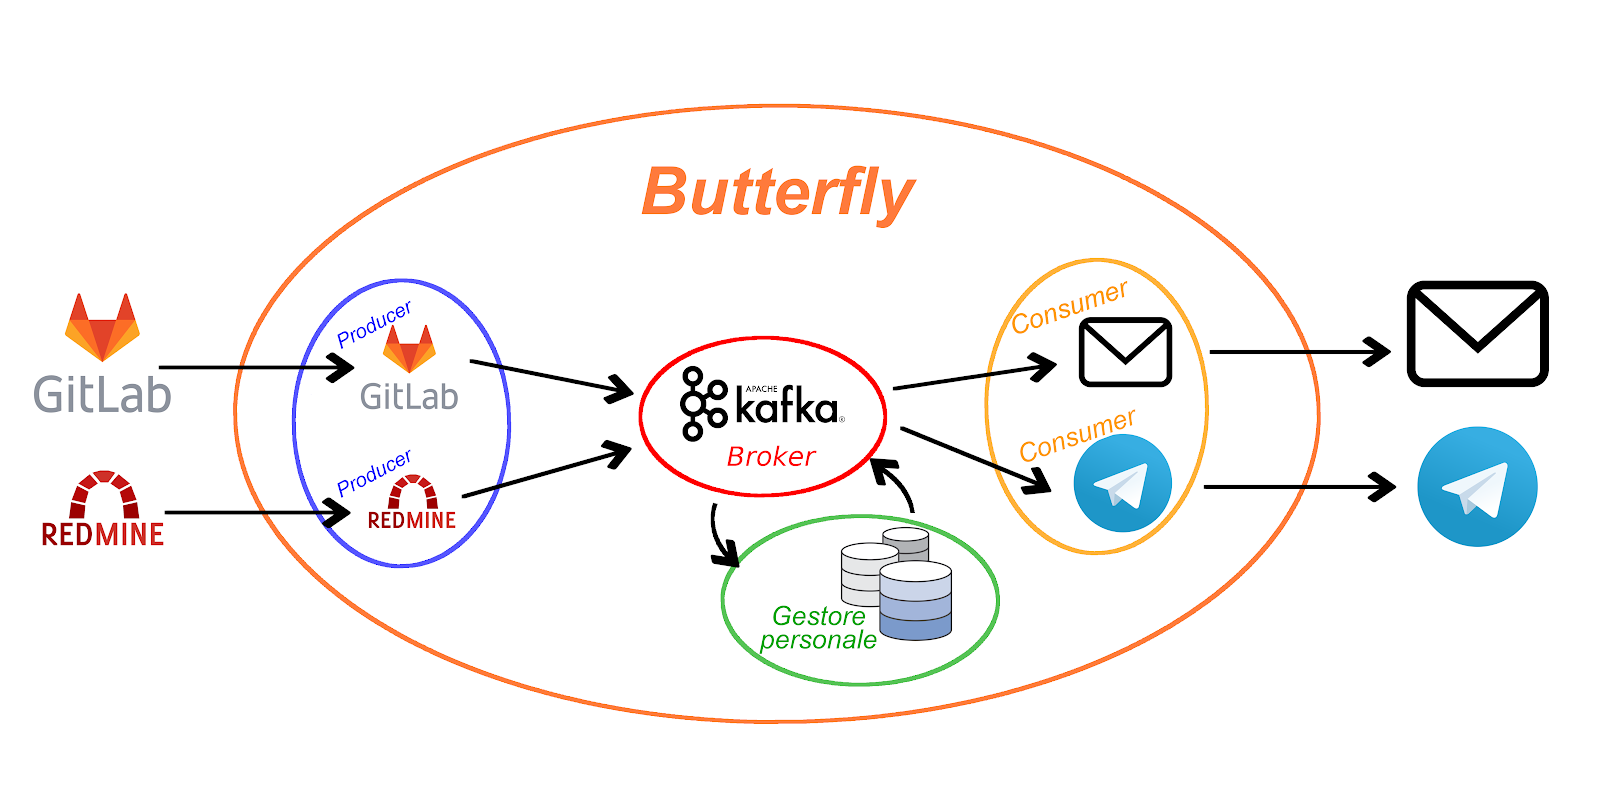
\includegraphics[width=\textwidth]{img/butterfly.png}\\
    \caption{Visione generale di \progetto}
    \label{fig:butterfly}
\end{figure}
